\documentclass[12pt]{article}
\usepackage[utf8]{inputenc}
\usepackage[T1]{fontenc}
\usepackage[english]{babel}
\usepackage{csquotes}
\usepackage{microtype}
\usepackage[font=small,labelfont=bf]{caption}

\usepackage{dirtytalk}

\usepackage[draft]{graphicx} %TODO: hier das "draft" rausnehmen

\usepackage{pdfpages}

\usepackage[marginpar]{todo}

\usepackage{etoolbox}
\AtBeginEnvironment{quote}{\small\setstretch{.25}}

\usepackage[scaled]{helvet}
\renewcommand{\familydefault}{\sfdefault}

\renewcommand\labelenumi{(\theenumi)}

\usepackage[style=authoryear-icomp,maxcitenames=2,backend=biber]{biblatex}
\DefineBibliographyStrings{english}{ 
   andothers = {{et\,al\adddot}},             
}
\addbibresource{bibliography.bib}

\usepackage{titlesec}
\titlespacing\section{0pt}{12pt plus 4pt minus 2pt}{0pt plus 2pt minus 2pt}
\titlespacing\subsection{0pt}{12pt plus 4pt minus 2pt}{0pt plus 2pt minus 2pt}
\titlespacing\subsubsection{0pt}{12pt plus 4pt minus 2pt}{0pt plus 2pt minus 2pt}

\usepackage{setspace}
\usepackage{color}
\definecolor{hgray}{gray}{0.5}

\usepackage{enumitem}
\setlist[itemize]{noitemsep, topsep=0pt}
\setlist[enumerate]{noitemsep, topsep=0pt}

\usepackage[hidelinks,
pdfpagelabels,
pdfstartview = FitH,
bookmarksopen = true,
bookmarksnumbered = true,
linkcolor = black,
plainpages = false,
hypertexnames = false,
citecolor = black] {hyperref}


\usepackage{geometry}
\geometry{
  left=2.5cm,
  right=2.5cm,
  top=2.5cm,
  bottom=2cm,
  bindingoffset=0mm
}
\usepackage{wrapfig}

\usepackage{listings}
\lstset{language=HTML,keywordstyle={\bfseries \color{blue}}}

\makeatletter
\title{Twitter analysis for laymen: Using Big Data and Visualisation to understand Twitter discussions}\let\Title\@title     %   Titel der Arbeit eintragen
\makeatother

\usepackage{fancyhdr}
\usepackage{afterpage}
\fancypagestyle{MRstyle}{%
    \fancyhf{}
    \fancyhead[L]{\textit{\textcolor{hgray}{\Title}}}
    \fancyfoot[c]{\textcolor{hgray}{\thepage}}
}
\pagestyle{MRstyle}

\fancypagestyle{appendix}{%
    \fancyhf{}
    \fancyhead[L]{\textit{\textcolor{hgray}{\Title}}}
    \fancyhead[R]{\textcolor{hgray}{\rightmark}}
    \fancyfoot[c]{\textcolor{hgray}{\thepage}}
}

\usepackage[hang]{footmisc}

\usepackage{parskip}

\newcommand\fakesection[1]{% 
    \markboth{#1}{#1}}
    
\usepackage{subfiles}


\begin{document}
%\pagestyle{MRStyle}

\setstretch{1.15}

\begin{titlepage}
    
    \large
    RWTH Aachen\\
    Lehrstuhl für Communication Science\\
    Prof. Dr. M. Ziefle
    
    \vspace{5cm}
    \Large
    \doublespacing{
        \textit{Master thesis\\}
        \textbf{\Title}
    }
    
    \vspace{7cm}
    \normalsize
    \setstretch{1.2}
    by:\\
    Martin Schmitz (Matrikel-Nr.: 320669)\\
    Phone: +49 163 8562072\\
    martin.schmitz2@rwth-aachen.de
    
    \vfill
    
    Aachen, \today    
\afterpage{\cfoot{\textcolor{hgray}{\thepage}}}
        
\end{titlepage}

\pagenumbering{Roman}

\tableofcontents

\clearpage

\pagenumbering{arabic}
\section{Introduction}
Humans have always communicated (\cite{tomasello2010origins}). Over the centuries, this communication evolved and became more complicated. What began with hand gestures evolved into myriads of spoken and written languages.

At the same time, the target audience of communication grew. From small, tight-knit communities, to larger ones, to one-sided mass media communication which allows single actors to reach millions of people (\cite{luhmann1995realitat}). Over the last few years, yet another form of communication emerged. Social networks combine traditional, multi-sided communication with the range of mass media and change the way people communicate with each other: behavioral patterns that were formerly mostly seen in celebrities are now adopted in regular interpersonal communication on social media sites (\cite{stefanoneRelationshipTraditionalMass2010}).

This opened communication empowered people to look up information for themselves, rather than having to rely on a single expert in their community. However, the internet is riddled with information with bad quality. These low-quality information can spread misinformation and lead to skepticism towards scientifically proven concepts (\cite{krimskyRiskCommunicationInternet2007}). One famous example for this is the wide-spread misinformation that vaccines cause autism---a myth that has been debunked multiple times, but gets still spread via the internet (\cite{baker2008mercury}).

The often outrageous nature of these kinds of content often drives engagement: one study showed that anti-vaccine contents got retweeted 4 times as often as neutral tweets about vaccinations (\cite{blankenshipSentimentContentsRetweets2018}). As the big players on the Internet---Google, Facebook, and Twitter---make money off of this engagement, it is in their interest that users see as many engagement-driving contents as possible. This leads to recommendation algorithms which show these contents again and again to people susceptible to this kind of (mis-)information.

This leads to the so-called \emph{filter bubble-effect}. The opinion a user already has gets enforced (\cite{pariser2011filter}), while opposing facts or opinions are less visible. This can lead to social problems: Discussions become less diverse and people think they are part of the majority, even if they are part of a loud minority (\cite{moscoviciSilentMajoritiesLoud1991}).

As of now, Social Networks do not offer a transparent look into their recommender algorithms. This means that users cannot be sure whether their opinion is actually shared by a majority. One way to fight this problem is Big Data (\cite{crawfordCriticalQuestionsBig2012}).

As its name suggests, Big Data relies on huge datasets to give meaningful results and insights. Generating these data sets manually is a challenge that is virtually impossible. However, Twitter allows the automated collection of tweets via their APIs. This means that data collection can run fully automated over a prolonged time. Leveraging such a data set could give user's a bird's-eye view on the social network so that they could see for themselves how certain discussions are unfolding. For this, data visualizations play a big role, as they can help making huge data sets accessible to laymen (\cite{donalekImmersiveCollaborativeData2014}).

This thesis aims to answer two questions:

\begin{enumerate}
    \item Is it possible to automatically collect all German-language tweets about a specific topic, and store these tweets in a way that they can be analyzed?
    \item Can this data be processed and visualizied so that laymen can gain insight from this data?
\end{enumerate}

For this, an app that automatically tweets about the currently ongoing corona epidemic was written. Then, interactive data visualizations for this data were coded. Lastly, these visualizations were tested with laymen who had little to no experience working with big data sets.


\clearpage
\section{Related work}
This part reviews and compiles work that has already been done on Twitter analysis, big data, and visualization. It discusses the influence Twitter has on communication nowadays, explores work that has been done regarding automatic data collection on Twitter, and shows ways to construct a meaningful data visualization.

\subsection{Twitter as a microblogging platform}
The microblogging platform \emph{Twitter} allows users to post messages that are up to 280 characters long, so-called \emph{tweets}. Users can follow other users; each user's timeline is then populated by tweets of people they follow (\cite{thimmTwitterAlsWahlkampfmedium2012}). Accounts can also be verified. This \say{lets people know that an account of public interest is authentic} (\cite{twitterinc.VerifiedAccounts}).

Seeing that Twitter users share their opinions on many topics openly, the platform offers a good data source for researchers to assess the public's opinion (\cite{pak2010twitter}, \cite{pfaffenberger2016twitter}, \cite{broniatowski2014twitter}). Twitter also has a very diverse audience: Politicians and journalists are using the platform the same way as celebrities or regular users (\cite{pak2010twitter}), which lets researchers collect data from different social groups and groups with diverse interests.

As opposed to other social networks, like Facebook, users can view tweets by all\footnote{By default, Twitter accounts are public. Users can set their profile to private, which means that only accepted followers can see their tweets} instead of only by those who are in their network (\cite{parkDoesTwitterMotivate2013}). While Facebook focuses on building a network of real-life friends and keeping in touch with them, Twitter nudges its users to voice their opinions publicly by choosing default settings for the user that supports this kind of usage. The Twitter page of a user and the page of a multi-national business conglomerate share the same functionality from the beginning, while Facebook differentiates between personal pages and public-facing pages.

Twitter is a medium that is widely used by the 'ordinary public', which means that people without celebrity status can use it as a platform to find an audience. A 2011 study conducted in South Korea examined the most popular 1\% of tweets. The researchers found out that the majority of those tweets were sent by people without celebrity status (\cite{chang2011structure}, as cited in \cite{parkDoesTwitterMotivate2013}).

Thus, Twitter is also a suitable survey tool. Collecting data from Twitter eliminates problems that classical surveys have, like low sample size or selection bias (\cite{takabeTwitterSurveyTool2016}). The low sample size is not a problem because of the high number of Twitter users, which was 330,000,000 by the beginning of 2019 (\cite{TwitterMonthlyActive}). The selection bias is circumvented because researchers are no longer active recruiters who look for participants. They are almost passive consumers of already existing data instead. Nevertheless, one has to keep in mind that the community of Twitter users is not necessarily representative, as internet access, affinity to social media, and so forth varies. %TODO: Add TAM or similar source here?

Because of Twitter's unique ability to reflect the thought processes of individuals, some scholars say that Twitter should be documented and archived as a historical record (\cite{risse2014documenting}). Twitter documents today's society in great detail---and, more importantly, individuals document their own experiences. This is a stark contrast to (historic) documentation in the past, where no direct documentation happened. There was always an intermediate between the individual who experienced something and the documentation (\citeauthor{risse2014documenting}).

Scholars who are in favor of archiving Twitter argue that not only the text of a tweet is important, but also the context, like who sent the tweet and at what time. They also argue that further natural language processing is needed to search an archive for specific topics. This necessary natural language processing is no easy task on Twitter. Due to the 280-character-limit (which used to be 140 in the beginning years of Twitter, but was since doubled), many vernaculars and abbreviations are used, which can be difficult for natural language processors to process. Nevertheless, the authors claim that \say{Twitter can be seen as a comprehensive documentation of society} \parencite[9]{risse2014documenting}, and say that this documentation can be of immense historical value for future generations.

\subsection{Twitter as a news source}  % Maybe "Twitter and crowd journalism" or something?
When Osama bin Laden was killed, the information was spread via Twitter before it hit major news outlets (\cite{hu2012breaking}). \citeauthor{hu2012breaking} analyzed the certainty of tweets that were sent between the first rumors of the killing and the official confirmation. This certainty analysis showed that many people were already sure that this news was true before officials confirmed it. \citeauthor{hu2012breaking} concluded that people saw Twitter as a trustworthy source for these breaking news. The bin Laden killing is thus one of the earliest reported cases of Twitter being faster than traditional media, but equally accepted as a trustworthy source (\cite[2751]{hu2012breaking}).

A study examining the social media-usage around the protests of the 2010 G20 summit in Toronto shows that Twitter is a suitable platform for crowd-sourced journalism (\cite{poell2012twitter}). Crowd-sourced journalism, or alternative journalism, positions itself as the opposite of mainstream journalism. According to the authors, mainstream journalism often focuses on the events themselves, like demonstrations or riots, instead of the underlying issues that people are protesting against. Opposed to that, crowd journalism has the chance to shine a light on why people are protesting, by making these people heard (\cite[698]{poell2012twitter}). 

This study from 2012 analyzed the usage of three different social media platforms during the G20 protests: Twitter, YouTube, and Flickr. Of the three platforms the researchers examined, Twitter was used by most people, and the retweeting-feature gave more silent users the possibility to weigh-in without having to create their content (cf. \cite[709]{poell2012twitter}). However, the authors concluded that the content published on social media-platforms was focused on sensationalist messages, similar to how mainstream journalism operates. Instead of focusing on the meaning of the protests, and the motivation of the protesters, the focus lay again on sensationalist pictures. This goes against the intention of crowd-sourced journalism.

Using social media in as a reliable source for news and knowledge even affected the 2016 election of the US president (\cite{duttSenatorWeSell2018}, \cite{ribeiroMicrotargetingSociallyDivisive2019}). During this election, Russia allegedly bought microtargeted ads on Facebook which appeared on users' newsfeeds as regular posts with a small tag claiming that this was paid content. These paid ads often contained false information about the democratic party and their candidate, Hillary Clinton. Researchers came to the conclusion that these ads, specifically targeting key demographics which could have swung the vote against Trump, tampered with the outcome of the election in Russia's favor.

\subsection{Filter bubble in social networks}
While social networks can connect people all over the world, scientists believe that their recommender algorithms are designed in a way that amplifies users' own opinions instead of connecting users with opposing views to generate healthy discussions (\cite{pariser2011filter}). \citeauthor{pariser2011filter} coined the term of the \emph{filter bubble}. His thesis is that those recommender algorithms select content for users that they mostly agree with. This traps users in a bubble where they are rarely confronted with opposing worldviews, as Google searches, the Twitter timeline, Facebook, Instagram, Reddit, and the likes mostly recommend contents that adhere to their world view---without the users' consent or even knowledge.

This leads to worries about online discussions becoming less diverse. Rather than exposing their users to a plethora of viewpoints and arguments, social media platforms and search engines decrease information diversity to improve engagement on their websites (\cite{bozdagBreakingFilterBubble2015}). One study found out that especially in political issues Twitter users tend to communicate mainly with users who share their political views (\cite{barberaTweetingLeftRight2015}). In a filter bubble, the own opinion seems to be shared by the majority of people---even if one is part of a vocal minority.

How big the effect of the filter bubble on the culture of discourse is remains unclear (\cite{brunsEchoChamberWhat2017}). A study examining the Australian Twitter-sphere has found that while there are some clusters of Twitter users, \say{those connections have not been made to the exclusion of all others} (\cite[9]{brunsEchoChamberWhat2017}). This means that while there are distinct groups of users that are all strongly connected, those clusters are still connected. Users from these clusters have connections to people \emph{outside} their cluster: From a network-centric view, this indicates that filter bubbles don't exist, as distinct clusters would have little to no connections between each other. However, this study fails to incorporate Twitter's default news feed which shows algorithmically picked posts first rather than a chronological timeline of all activity in a network. Even though people follow other people they do not necessarily agree with, the recommender algorithm might only show tweets by others they agree with. The study also does not take into account \emph{why} people followed accounts outside their cluster. 

One survey conducted in the UK showed that politically interested users know about filter bubbles and actively try to avoid them (\cite{duboisEchoChamberOverstated2018}). The participants of this study reported that they actively choose to read some media outlets which they know they do not agree with. \citeauthor{duboisEchoChamberOverstated2018} conclude that people who are politically interested and have a diverse media diet can prevent themselves from getting caught in a filter bubble and thus keep a broader look on ongoing discussions. Seeing that the results come from a survey where participants self-reported their behavior and their internet usage, it is unclear if these users manage to avoid the filter bubble: \citeauthor{bozdagBreakingFilterBubble2015} pointed out that users are usually unaware that their content is filtered. 

The fact that social networks influence people's opinions can become problematic because people can adapt their opinion to match these of opinion leaders (\cite{altafiniDynamicsOpinionForming2012}). \citeauthor{gokceTwitterPoliticsIdentifying2014} describe opinion leaders in the following way:

\begin{quote}
    (Opinion leaders are people) whose ideas have a continuous presence and following in conventional, and—more recently—in electronic media. Newspaper columnists, non-governmental organization leaders, prominent politicians, and public intellectuals (\emph{and sometimes popular media figures}) fall into this category (\cite[673]{gokceTwitterPoliticsIdentifying2014}, emphasis by the author.)
\end{quote}

Adapting one's opinions to those of popular media figures may mean to accept someone as an authority in a field where he or she has no formal education and is unknowingly spreading false information. The opinion leadership of media figures, paired with the effect of the filter bubble, could lead to a less-informed minority who see themselves as a well-informed majority (\cite{moscoviciSilentMajoritiesLoud1991}). This could potentially lead to a political polarization of users (\cite{kobayashiDepolarizationSocialMedia2020}).

%It appears as if Twitter is, on the one hand, a grassroots medium, allowing the broader public to engage in discussion and form an opinion

\subsection{Looking past the bubble using big data}
As previously discussed, the filter bubble may prevent people from acknowledging that their viewpoint is not the universal truth, as well as leading to the false impression that they represent a majority of people. As this effect is mainly driven by the content recommendation algorithms inside the network, and individual users have little to no control over which content these algorithms show to them, it may be impossible to get a clear, unbiased view as a user from inside the network.

One way to empower users to look beyond their bubble is to give them a bird's eye view of Twitter. Twitter's API can be used to automatically collect all publicly available tweets that match certain search criteria given by the user (\cite{twitterinc.TwitterAPIs}).

The API allows easy access to tweets and provides functionality to filter tweets by keywords, hashtags, language, or geographic regions (\cite{bello2017detecting}). This allows scientists and coders to get a nearly full overview, unbiased by recommendation algorithms or personal preferences. Twitter offers two different ways to access tweets via their API:

\begin{enumerate}
    \item \textbf{The Archive API} gives access to Twitter's archives up to the past 30 days. Users can search for tweets matching specific criteria and retrieve them from the archive.
    \item \textbf{The Streaming API} streams new tweets that match given criteria to a specified endpoint as soon as this tweet is sent. New contents immediately reach the endpoint, however, content that has already been sent before the data collection started cannot be retrieved using this API.
\end{enumerate}

Collecting data automatically via Twitter's API is not without its flaws, though. Over the last years, Twitter has implemented a premium model for its API; due to the high costs for the premium access, scholarly research on Twitter has been limited (\cite{brunsTwitterDataWhat2014}). One example of the limitations is that the free API plan only gives access to 1\% of the total current volume on Twitter. If 100,000 tweets are sent per minute over all of Twitter, the API would only give access to at most 1,000 tweets matching the query. Using the Streaming API gives access to all tweets matching the given criteria in a given moment; however, access to Twitter's archives is impossible using this stream. This makes it necessary for researchers to set up own databases and collect data over a prolonged time.

Collecting such big amounts of raw data is commonly called working with \emph{Big Data} (\cite{crawfordCriticalQuestionsBig2012}). This term used to refer to data sets that were so big that you needed a supercomputer to use them; \citeauthor{crawfordCriticalQuestionsBig2012} noticed, however, that the name nowadays carries technological, analytical, and mythological components. Big Data does not only mean bigger data sets, but also carries a 

\begin{quote}
    widespread belief that large data sets offer a higher form of intelligence and knowledge that can generate insights that were previously impossible, with the aura of truth, objectivity and accuracy. (\cite[3]{crawfordCriticalQuestionsBig2012})
\end{quote}

This belief seems to be summed up in the equation 'more data = more insight'.

Manually analyzing these amounts of data is virtually impossible, but luckily, the last few years brought big advances in natural language analysis. Automated natural language analysis can be used to understand and explain social behavior in text-based social networks.

\citeauthor{bahk2016publicly} developed a prototype for a dashboard that helps to monitor the population's sentiment toward vaccinations. The so-called 'anti-vaxxers' pose a real threat to the wider population because vaccines only work effectively if a majority is vaccinated. Thus, it is interesting to know when and where negative sentiment towards vaccinations arises to formulate countermeasures, like targeted information campaigns. The authors searched Twitter for vaccine-related messages and automatically calculated the sentiment of those tweets. The generated data is presented on a dashboard, which shows the negative sentiment per country, along with further filters. According to the authors, \say{[the dashboard] can be used to detect early signals in shifting conversations about vaccination} (\cite[343]{bahk2016publicly}). Users of this dashboard can see in which regions vaccinations are particularly frowned upon, and can then continue to formulate said countermeasures.

Another study found that Twitter is a useful source for measuring climate change awareness (\cite{codyClimateChangeSentiment2015}). The authors of this study developed a so-called \say{Hedonometer} that they use to compute a happiness-score for tweets. First, they used Amazon's \emph{Mechanical Turk} service to let people rate words in a corpus on a scale from 1--least happy to 9--most happy. Then, they removed neutral or ambiguous words which scored in the middle of the scale, between 4 and 6, from the corpus. This annotated corpus was used to compute the overall happiness of a tweet. With this set of happiness-scores for tweets, \citeauthor{codyClimateChangeSentiment2015} mapped out the average happiness of tweets that contained the word \emph{climate} compared to the average happiness of all collected tweets. This gave the authors an unfiltered insight into how the general public perceives climate change and the surrounding discussions.

\citeauthor{weberInterdisciplinaryOptimismSentiment2019} also collected tweets automatically to find out how researchers experience interdisciplinary research. For this, they collected tweets that contained the words \emph{interdisciplinary}, \emph{transdisciplinary} and \emph{multidisciplinary} using the Twitter API. After they collected the dataset, they pre-processed it to remove duplicated tweets and retweets, as well as lemmatization, removing numbers and punctuation, and other common pre-processing steps for natural language processing. After this, they trained a machine learning classifier using several publicly available annotated datasets. This classifier then categorized tweets in three categories: \emph{positive}, \emph{neutral}, and \emph{negative}.

They found out that negative tweets did not only contain tweets that were critical against interdisciplinary studies, but also tweets that depicted every-day hardships scientists have to struggle with, like rejected peer-reviews and difficulties in securing funding. Neutral tweets were most often job postings, calls for applications, or announcements for new publications. Positive tweets were often about conferences and workshops, but also about the method of interdisciplinary research itself. Most of the tweets collected in this study were classified as neutral (\cite[7]{weberInterdisciplinaryOptimismSentiment2019}).

% Idee dieser Subsection: Erklären, was alles dadurch erreicht werden kann, dass NLA auf Tweets angewandt wird. Beispiele: Vaccination Dashboard, rausfinden dass anti-vaccine tweets häufiger retweetet werden als pro-vaccine tweets

\subsection{Visualizing big data}
In the last couple of years, we generated more data than in the combined history of humankind (\cite{helbing2019will})---and with the Internet of Things on the rise, experts assume that the amount of data will double every 12 hours.

The more data we collect, the more important it becomes to understand big data (\cite{bornerDataVisualizationLiteracy2019}). The most common form to store such big data is in databases, which usually show data in big tables. However, data in tabular form is exceptionally hard to read for humans. As human perception is fine-tuned to recognize underlying patterns, trends, and outliers, \emph{Data Visualization} is one of the most common tools to explore and communicate big data sets (\cite{heerTourVisualizationZoo2010}). Recognizing trends helps with understanding what the data set is telling in general, while outliers help to find cases that could require further attention and detail.

Visualizations help to make sense of big data in a more intuitive way than reading database tables or big charts (\cite{donalekImmersiveCollaborativeData2014}). As data-driven decision-making becomes more and more important (\cite{brynjolfssonStrengthNumbersHow2011}), the ability to read and construct data visualizations will become an important skill in the future.

But even though data visualizations are known to help people understand big data sets, studies have shown that laymen often do not have the required knowledge to accurately read complex visualizations (\cite{bornerInvestigatingAspectsData2016}). This means that data visualizations have to be constructed carefully and assume almost no previous knowledge when it comes to providing explanatory texts or supporting elements in the visualizations. As \citeauthor{bornerInvestigatingAspectsData2016} have shown, laymen can read the most basic kinds of data visualizations, like bar charts and line charts. However, even for those well-known charts, participants had trouble naming and interpreting the visualizations.

Thus, data visualization is not inherently self-explanatory. Our ability to extract information from visualizations and answer questions based on data sets is called \emph{Data Literacy} (\cite{boyPrincipledWayAssessing2014}). Improving this literacy allows people to not only improve their communication and collaboration on data sets, but also their understanding of the world as shown by big data (\cite{bornerDataVisualizationLiteracy2019}).

At the same time, a good data visualization is flexible and does not provide definite answers in itself. It should rather support users to answer their own questions (\cite{light2001portable}). To enable users to do this, \citeauthor{shneidermanEyesHaveIt1996} formulated a Visual Information Seeking Mantra:

\begin{quote}
    Overview first, zoom and filter, then details-on-demand (\cite[337]{shneidermanEyesHaveIt1996})
\end{quote}

\emph{Overview first} means that a data visualization should give an overview of the full dataset as a starting point, without any filters applied. The second step, \emph{zoom and filter}, means that users should have the possibility to zoom in on interesting items and rid the dataset of items that are not interesting for the user. Finally, \emph{details-on-demand} means that selecting an item should give further interesting details and concrete attribute values of this specific item that are not shown in the visualization itself. Showing users these details on demand, instead of visualizing every attribute, results in a less-cluttered visualization that is easier to understand.

The open-ended nature of data visualizations makes it challenging to measure the insight that users gain from data visualizations (\cite{northMeasuringVisualizationInsight2006}). One problem is that \emph{insight} is hard to define. \citeauthor{northMeasuringVisualizationInsight2006} gives five key characteristics to insight:
\begin{enumerate}
    \item \textbf{Complex,} which means that not only single data points are taken into account to measure insight, but all or at least most of the given data
    \item \textbf{Deep,} meaning that \say{insight often generates further questions} (\cite[6]{northMeasuringVisualizationInsight2006}) that in turn generate new insight
    \item \textbf{Qualitative,} meaning that the insight is not, e.g., an exact number, but more of an overall feeling
    \item \textbf{Unexpected,} with the author saying that insight is often creative and unpredicted, and
    \item \textbf{Relevant,} meaning that the insight goes beyond 'number-crunching' towards relevant results that affect the domain
\end{enumerate}
To measure these five dimensions, the author proposes to drop controlled experiments with benchmark tasks. These experiments often require very precise instructions for the participants which do not test insight very well as those tasks often result in yes/no-answers. Instead, \citeauthor{northMeasuringVisualizationInsight2006} says that complex benchmark tasks that are not closed questions help researchers measuring insight better. Benchmark tests could also be eliminated completely by focusing on qualitative analysis of the participants' performance. For this, participants could be asked open-ended questions without giving them concrete instructions how to find specific data in the visualizations. Participants are then asked to think aloud while solving the tasks. Their utterances can then be coded by the interviewers to map the answers on the five dimensions discussed above.


\clearpage
\section{Method}
This section explains how data was collected, how the different visualizations were coded, and how the candidates were tested.

\subsection{Data Collection Pipeline}
This section will go into further detail what data was collected from Twitter and how this data was collected, prepared, and stored.

\subsubsection{Fetching the data from Twitter} \label{sec:fetchedData}
The application for collecting the tweets was written in Python 3 (\cite{10.5555/1593511}), the Twitter API was accessed using the package \emph{Tweepy} (\cite{roesslein2020tweepy}). Tweepy's connection to Twitter's Streaming API was used to collect all German tweets containing one or more of the keywords
\begin{verbatim}
    Corona, Covid-19, covidioten, distancing
\end{verbatim}. From the returned Tweet Objects\footnote{The documentation on what data a Tweet Object contains can be found here: https://developer.twitter.com/en/docs/tweets/data-dictionary/overview/tweet-object}, only a few data points were kept that seemed interesting before the data collection started. This has mainly ethical reasons (\cite{richards2014big}). The author did not want to collect excessive personal data without having a good reason to, even though this has become the norm for big data over the last decade. The following data points of a tweet object get processed further and eventually saved to a database:

\begin{itemize}
\item \textbf{The full text of the tweet.} This is mainly used for sentiment analysis and other natural language processing-tasks.
\item \textbf{The tweet's time-stamp.}
\item \textbf{The ID of the tweet.} This makes it easier to check for duplicates in the data base. 
\item \textbf{The user name of the tweet author.} As discussed above, opinion leadership is a phenomenon also on Twitter. Collecting the user names allows for later analysis, e.g., which users tweet the most.
\item \textbf{The user's self-description.} Users on Twitter can enter a short description, the so-called \emph{bio}.
\item \textbf{The user's friend count.} This shows how many other accounts the user in question is following.
\item \textbf{The user's follower count.} This shows how many other accounts follow the user in question. \footnote{The definitions for a user's friend count and follower count can be found here: https://developer.twitter.com/en/docs/accounts-and-users/follow-search-get-users/overview}
\item \textbf{The country where the tweet was sent.} Twitter also offers coordinate-based geolocations, but choosing the country instead seemed to honor the user's privacy more.
\item \textbf{Whether the account is verified or not.}
\item \textbf{The source of the tweet.} This shows if the tweet came from the Web-App, a desktop app, a mobile app, a 3rd party-application or other sources.
\item \textbf{The calculated sentiment of the tweet.} The score gets calculated during the pre-processing of the tweet. Later sections will go into more detail on how the sentiment is calculated.
\end{itemize}

%TODO: Add figure how the data was collected (it's in miro)

Twitter's \emph{Streaming API} was used as it gives the most complete data set on Twitter's free tier (\cite{bruns2014}). It pushes (or streams) tweets that match the above-mentioned criteria to a specified endpoint the moment such a tweet gets sent on Twitter. An alternative to using the streaming API is to access Twitter's archive. However, the functionality of the archive is severly limited on the free tier of the Twitter API. Using the free tier, it is only possible to collect data from the last seven days, and even then the data set is not complete. Because of this, the streaming API was used in this study.

Using the streaming API meant, however, that the application had to run 24/7: the streaming API streams the data as it comes in and doesn't save it on Twitter's network. To ensure constant availability, the python application that connects to the streaming API and processes the incoming tweets runs in a Docker Container (\cite{merkel2014docker}) on Google's App Engine (\cite{google2020}). This made it easy to set up a server-less infrastructure with high availability.

\subsubsection{Data processing during the collection}
Every time the Streaming API sent a tweet to the app collecting the data, a sentiment score for the tweet text was calculated. For this, the Natural Language Toolkit (NLTK) was used (\cite{loper2002nltk}). NLTK uses a dictionary-based approach for sentiment analysis. This means that NLTK uses a corpus that is coded with different sentiment scores (\cite{haselmayer2017sentiment}). These scores are then summed up to calculate the overall sentiment of the tweet.
Compared with machine learning-approaches, this approach high precision, but low recall (\cite{soroka2015}). This means that the polarity of a sentiment as computed by NLTK is usually correct; however, many texts that do carry a specific sentiment are not recognized and are as such marked as texts with neutral sentiments.
A machine-learning-based approach for calculating sentiments was also considered. However, the tool would have required a server which runs a Java application. This would have meant a second instance of Google AppEngine, doubling the costs. Considering that the goal of this study is to test how laymen work with the dataset, and not a scientific analysis of the discussion about the coronavirus in the German twittersphere, the dictionary-based approach was chosen to keep down the costs.

\subsubsection{Storing the pre-processed tweets}
Tweets collected via the Streaming API are bundled to batches of 100. These batches then get published as a message to a \emph{Pub/Sub Topic}. According to Google, \say{Pub/Sub is an asynchronous messaging service that decouples services that produce events from services that process events} (\cite{google2020a}). In this case, collecting the tweets gets decoupled from writing the tweets to a data base. This approach has multiple advantages. For one, the database connection does not need to be open constantly. This makes the pipeline more robust: if the database connection is closed---for whatever reason---the messages published to the pub/sub topic is saved for up to 30 days. Once the database connection is re-established, the messages get ingested and the tweets are added to the data base. It also allowed for some early experimentation with the table schema for the SQL table. Pub/Sub could be configured so that already acknowledged messages stay in the system and can be fetched again. This meant that even though the table schema was constantly reset in the first couple of days of data collection, the data was not lost and could simply be re-fetched again.

The tweets are stored in a \emph{Google BigQuery} database, a server-less data warehouse that allows fast analysis of large amounts of data (\cite{google2020b}). \emph{Google Firebase} was also considered as data storage (\cite{google2020c}). As Firebase is a NoSQL database, the database queries would have been easier to write: Instead of using SQL, standard Javascript could have been used. This would have resulted in easier queries as Javscript features, like method chaining, would have been available. Seeing that the SQL-based BigQuery is better equipped to handle large amounts of data, this solution was chosen in the end. This turned out to be a good choice considering that the final dataset was almost 1GB big and that during an average testing session the data set was queried around 5 times. However, using BigQuery meant that the queries needed to be written in SQL, a language with complicated semantics (\cite{slutz1998massive}).

BigQuery was chosen over other SQL databases, like SQLite or Postgres, because it is also a Google service like AppEngine. This meant that authentication between the script collecting the tweets and the database did not have to be implemented. BigQuery can also be directly connected to a Pub/Sub-Topic using Google DataFlow. However, as the data were additionally processed, saving the data was handled in a dedicated script. 

\subsection{Visualizing the data}
To visualize the data from the streaming API, both Python libraries like ggplot (\cite{wickham2016}) and JavaScript libraries like D3 (\cite{bostock}) and VegaLite (\cite{uwidl}) were evaluated. To make the prototype as accessible as possible, a JavaScript based library was chosen, as JavaScript is a popular web technology. A web page is more accessible to laymen than a Python-based app, as there is no need to install additional tooling. And even though Python scripts, including visualizations, can be embedded easily on the web now, choosing a web technology seemed like the right approach.

Ultimately, D3 was chosen as a visualization framework. VegaLite is an opinionated framework which chooses many defaults for the user, while D3 is unopinionated. This means that the visualizations are harder to code but more versatile.

Early prototypes of the tool used a Svelte-based web page to show the visualizations. The final tool, however, was written in Observable\footnote{https://observablehq.com}. Observable is a JavaScript based notebook that, similarly to Jupyter Notebooks, combine code, output, and explanatory text. The notebooks allowed for quick iteration of the code, while its web-based nature also satisfied the requirement of being easily accessible without the need to download and install additional software.

\subsubsection{Fetching and processing the data}
While D3 can work with raw data input and perform, e.g., filtering operations on these inputs, data operations were performed directly in the database using SQL queries. This decision was made because the final dataset was almost 1GB big. Relying on D3 for filtering and aggregating the data would have meant that every time a user opens the tool, she would have to wait for the whole dataset to finish downloading before she could use the tool itself. Using SQL queries instead meant that a lot less data had to be sent to the tool: instead of downloading the full 997MB of the data set, the query results were only about 10KB big which greatly improved performance.

%To explore the dataset of collected tweets, users can have three additional filters that they can use
Users could explore the data using different filters:
\begin{enumerate}
    \item A word-filter which allows users to search the data base for tweets including a specific word.
    \item A toggle wether to include retweets in the data set.
    \item A toggle wether to include neutral tweets in the data set, with \emph{neutral} meaning tweets with a sentiment between -0.3 and +0.3). %TODO: write in related work about this
\end{enumerate}

The toggles to include retweets and neutral tweets in the data set changed the visualizations immediately, whereas the word-filter initiated a new database query. The idea behind this was that users are likely to look for a specific topic and then want to explore how this topic is presented in the data set. One possible scenario is that users want to find out how the general public thinks of masks. They then enter the keyword \emph{mask} into the search field and can then explore this topic further. The first version of the dashboard made a new database call every time one of the toggles was clicked. This became an issue during pre-tests: the delay caused by the database call made it difficult to compare the visualizations with the different filters, e.g., to compare how the graph looks with or without retweets included.

Because of this, data fetching was rewritten before the user tests started. Every time a user filters for a new word, the tool fetches the data for the four different filter permutations: the full dataset, the dataset without retweets, the dataset without neutral tweets, and the dataset without retweets and neutral tweets. If the user then toggles additional filters, the corresponding pre-fetched dataset gets immediately visualized instead of fetching a new dataset from the database.

\subsubsection{The visualizations themselves}
The final prototype that was tested included two different visualizations:
\begin{enumerate}
    \item \textbf{A visualization of the tweet volume over time:} Users can explore how many tweets were sent per day. When filtering for a word, users can see how many of the tweets per day contained the word they searched for. They can also toggle a normalized view which shows the percentage of tweets containing the search word, rather than the absolute number.
    \item \textbf{A visualization of the sentiment over time:} Using this visualization, users can explore if and how the public perception of a topic changed over time. This visualization also offers two views. The default view shows two lines: one line shows the sentiment for the tweets containing the search word, the other line shows the sentiment for the tweets \emph{not} containing the search word. A toggle shows only the daily average of all tweets instead, regardless of the search word.
\end{enumerate}

Time series were chosen as the primary visualization type because they are one of the most common visualizations (\cite{heer2010}). Choosing a common visualization aids laymen to read and interpret the data more easily (\cite{borner2016}), whereas more complicated visualizations can be difficult to understand for those people. Because of this, the development of certain aspects of the dataset \emph{over time} was chosen as the primary type of information that the visualizations should convey.

\begin{figure}[h!tb]
    \fbox{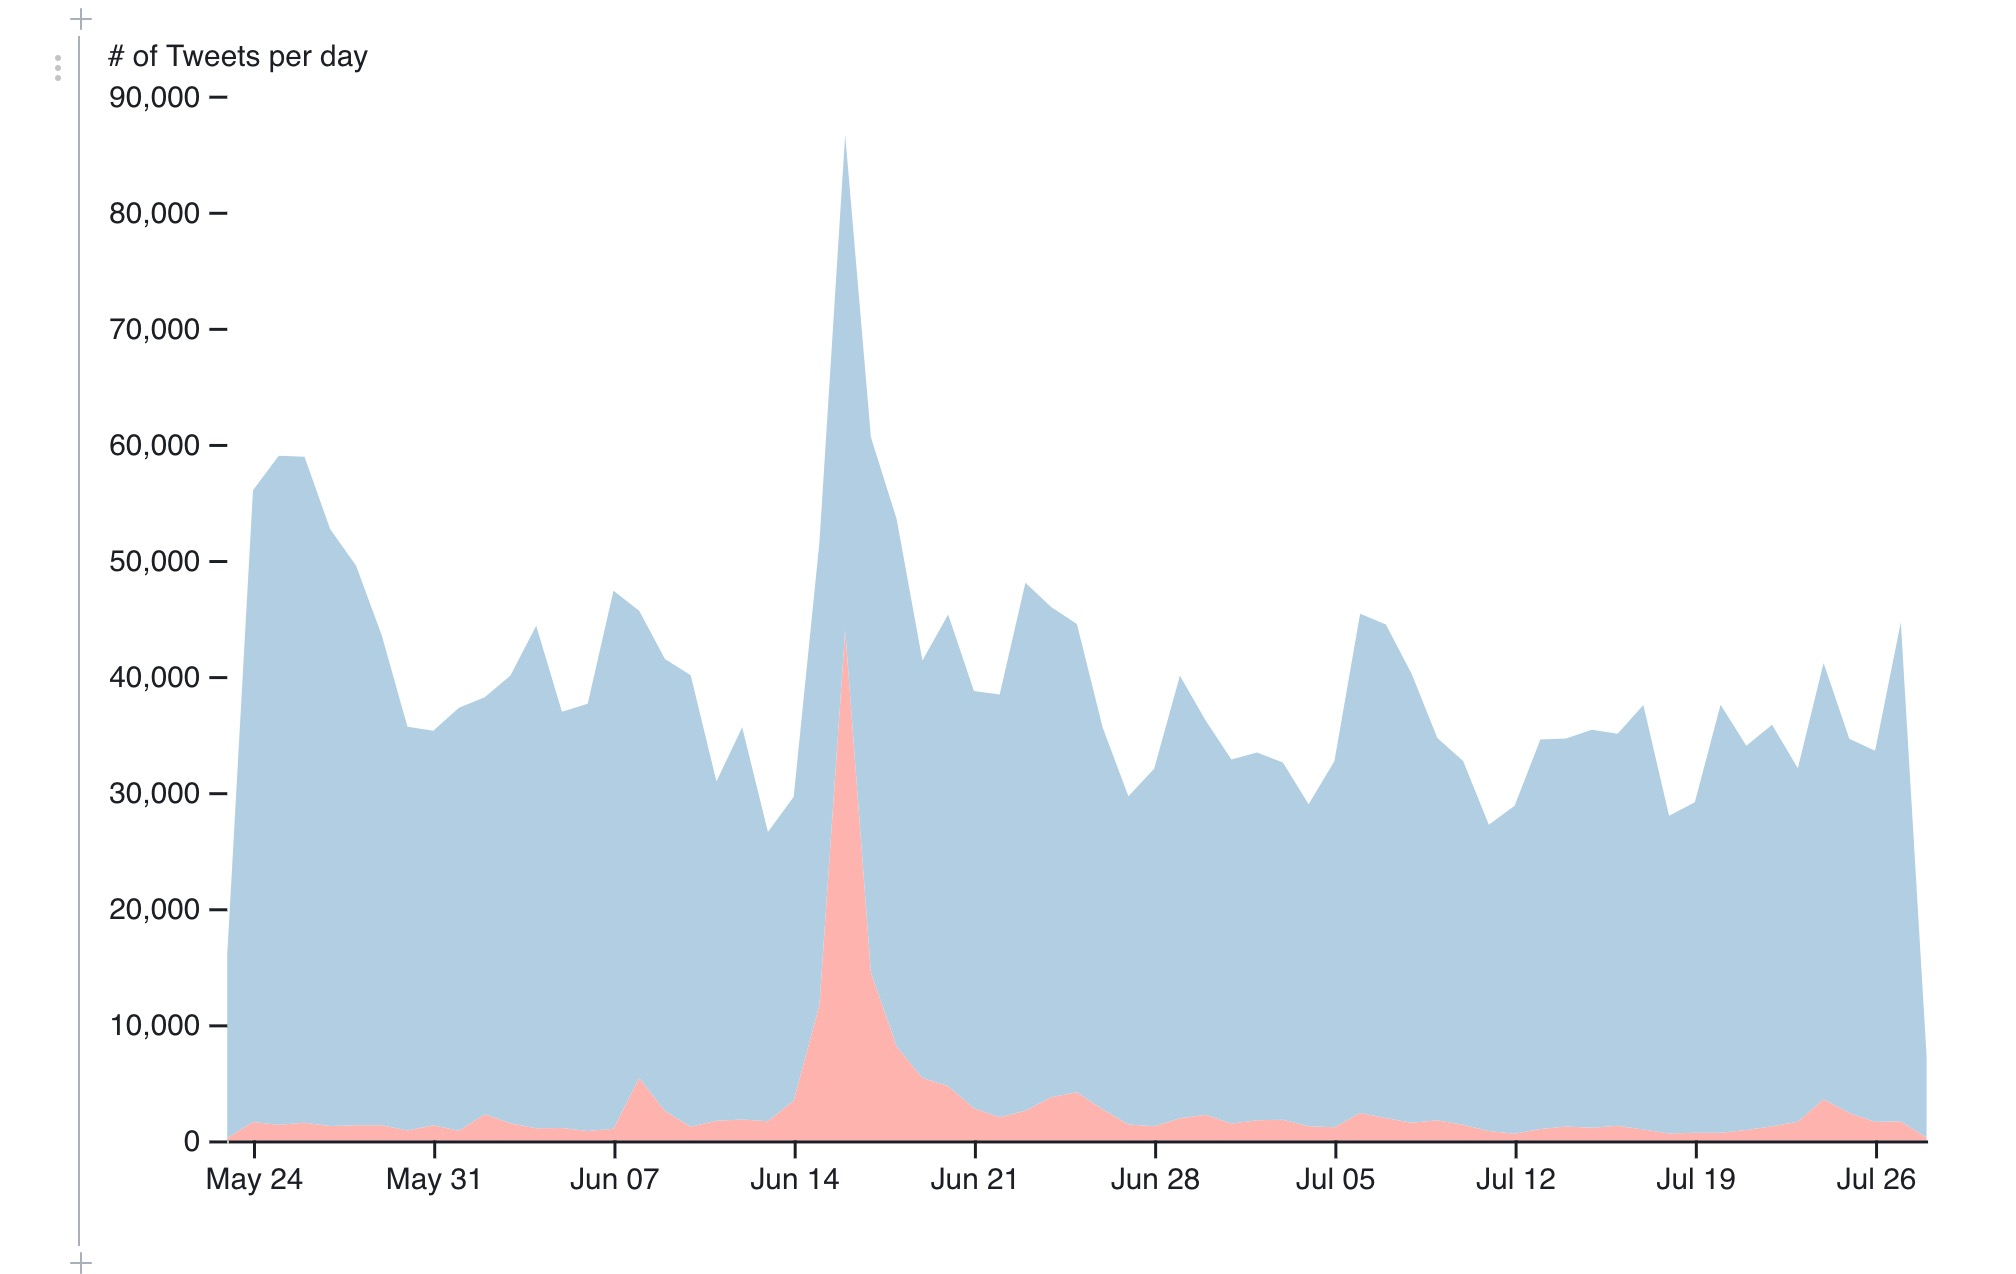
\includegraphics[width=\linewidth]{images/volume_areachart.jpg}}
    \caption{The daily tweet volume as shown in an area chart. This example shows the distribution of the word \emph{App}.}
    \label{fig:volume_areachart}
\end{figure}

To visualize the tweet volume over time, both an area chart and a bar chart were considered. Line charts and area charts are both common visualizations to show how something changed over time. Stock prices, for example, are usually shown as a line chart. An area chart is a line chart with its areas filled, which can be seen in figure \ref{fig:volume_areachart}. The filled area was used to indicate how many tweets contained the search word. However, visualizations which use line- or area charts to show development over time usually show data over a wider time range. For example, stock prices are usually shown over several years. The data set for this study spanned only around two months.

Because of this, the chart was changed to a bar chart, as seen in figure \ref{fig:volume_barchart}. Bar charts can't show information as concise as line charts or area charts. However, using a bar chart makes it easier to find and compare specific days. Using Chrome's responsive design inspector, the bar chart was pre-tested across multiple device sizes and appeared to be usable even on 11-inch displays without horizontal scrolling. The final user tests all used the bar chart visualization for the tweet volume.

\begin{figure}[h!tb]
    \fbox{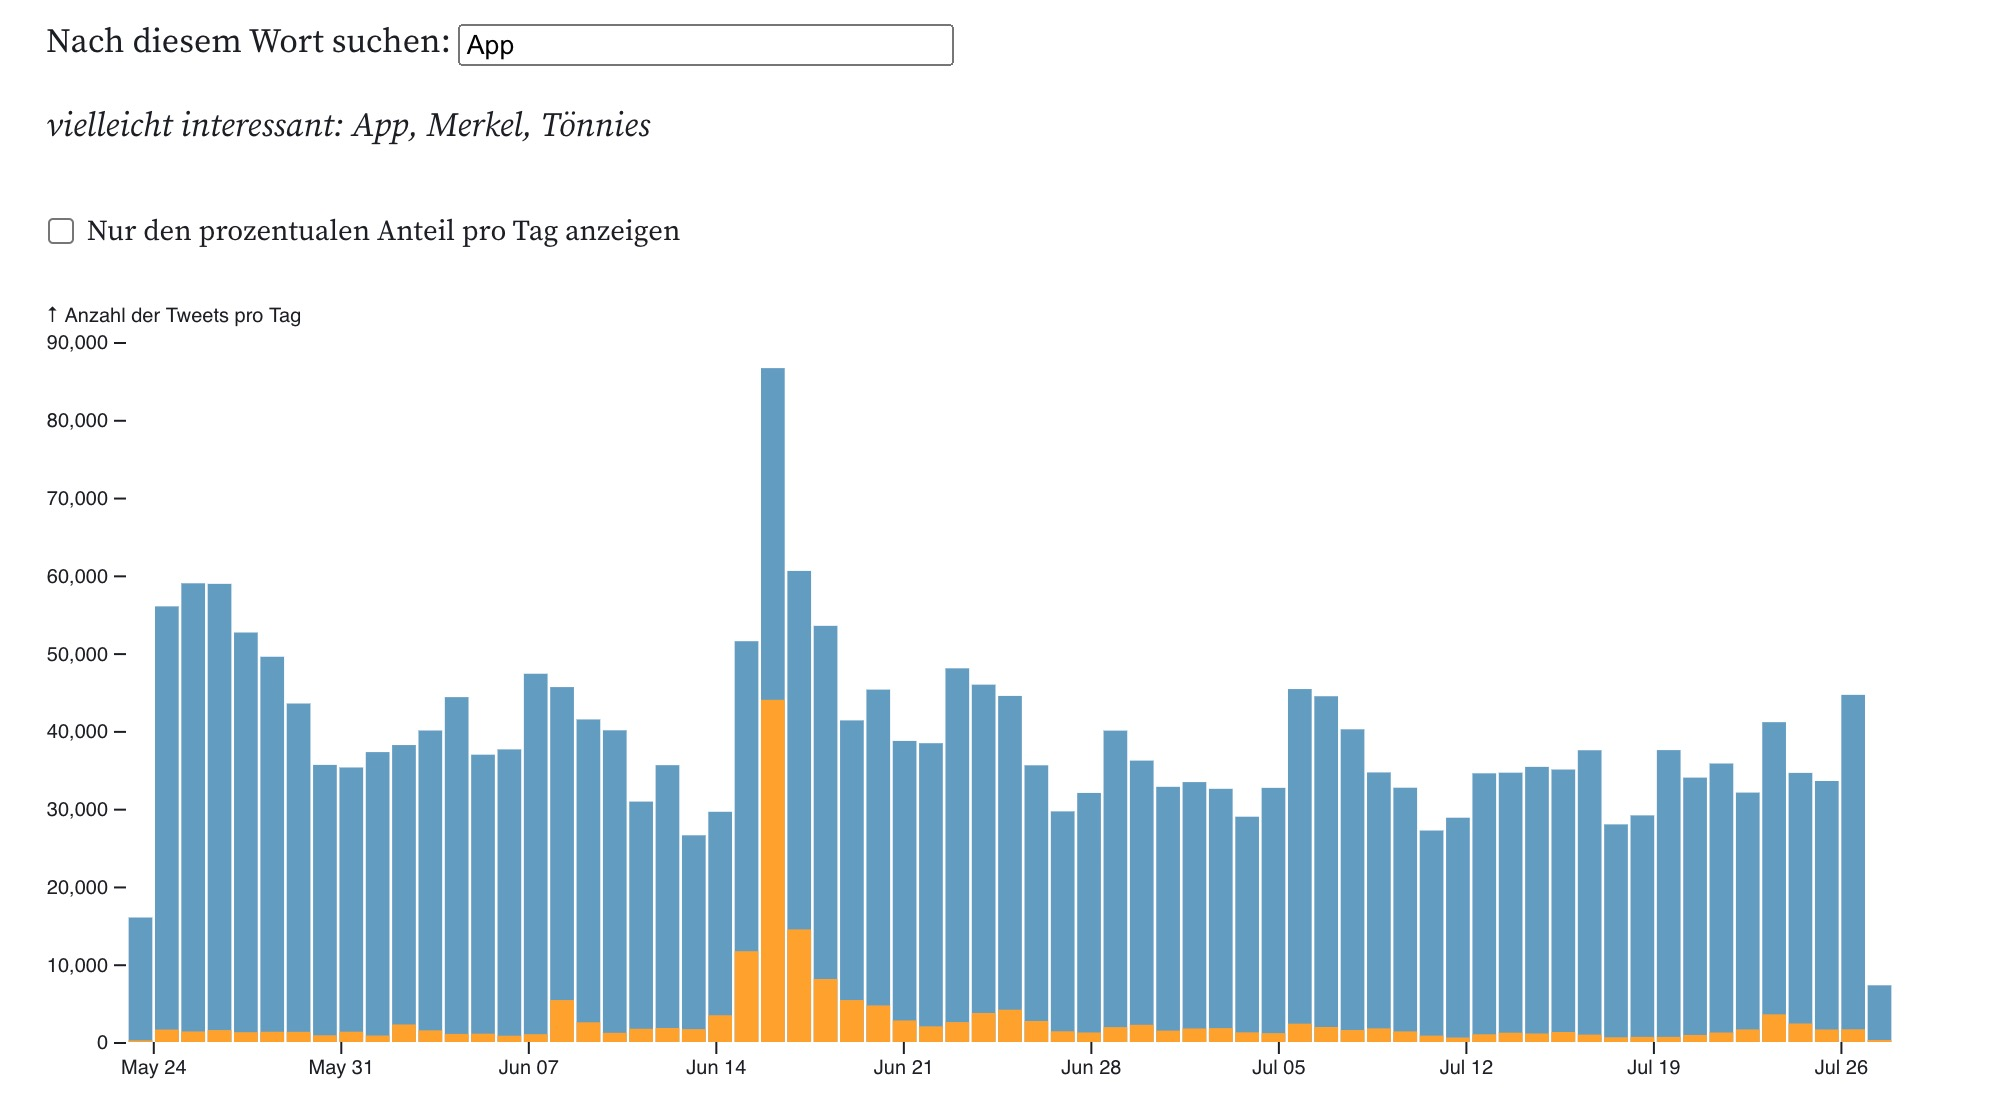
\includegraphics[width=\linewidth]{images/volume_barchart.jpg}}
    \caption{The daily tweet volume as a bar chart. This example shows the distribution of the word \emph{App}.}
    \label{fig:volume_barchart}
\end{figure}

The graph which shows the development of the sentiment over time is a line chart. This visualization was chosen because the sentiment can also show negative values, as its domain ranges from -1 to +1. 
% TODO Does this make sense? Why didn't I choose a bar chart? The line chart felt like the more natural choice here, but y tho?

\begin{figure}[h!tb]
    \fbox{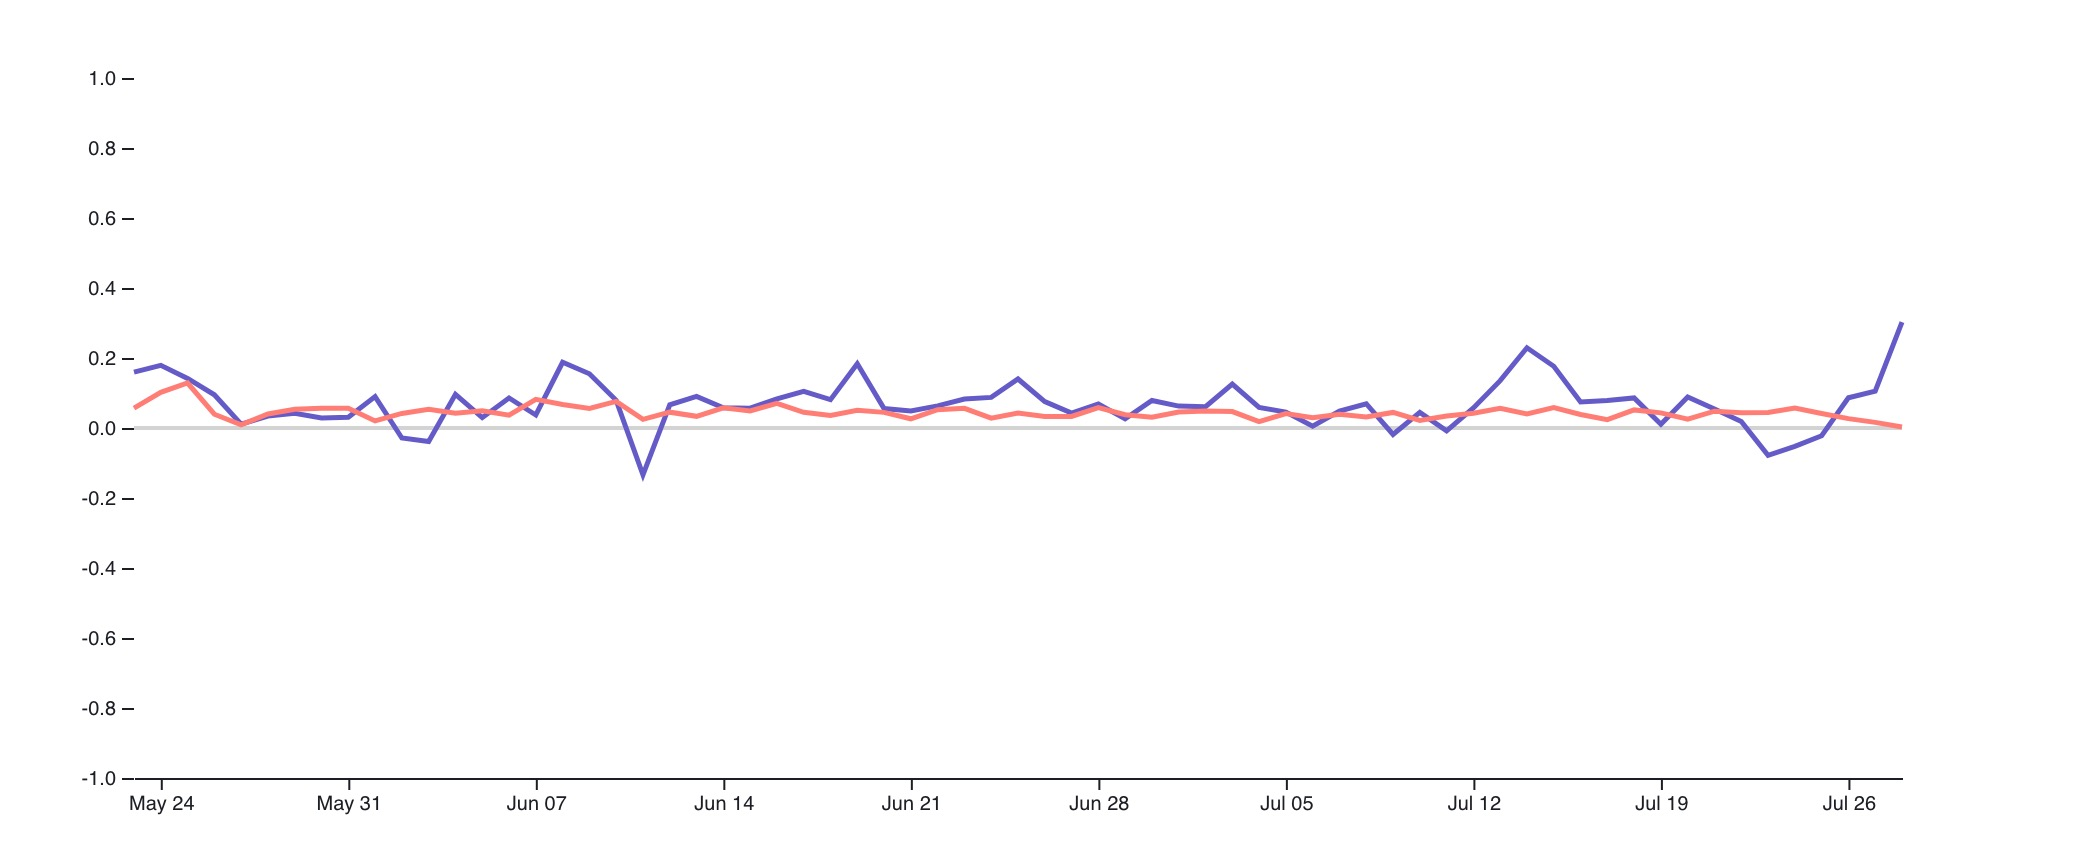
\includegraphics[width=\linewidth]{images/sentiment_linechart.jpg}}
    \caption{The average sentiment per day. The blue line shows the average sentiment of tweets containing \emph{App}, the red line shows the sentiment of tweets not containing this word.}
    \label{fig:sentiment_linechart}
\end{figure}

In this visualization, users can toggle between two view modes. The default mode shows the daily average sentiment of the tweets containing the search word as a blue line and the daily average sentiment of tweets \emph{not} containing the word as a red line. Users can also toggle to only see the average sentiment without any word-filters applied. This lets them, for example, see the influence of neutral tweets or retweets on the whole dataset.

The two visualizations share the same three aforementioned filters. This means that both visualizations share the same data set which could make it easier for participants to mentally connect them. At the same time, placing the filter possibilities at the top of the Observable notebook means that the visualizations are affected by filters that are not in their immediate neighborhood. This trade-off was tested in the user study which will be discussed later in this work.

\subsubsection{Ideas that were cut for time}
The big data pipeline and the visualization dashboard were both built using the principles of \emph{Shape Up}, a relatively new management approach for software development projects (\cite{singer2019}). The core principle of Shape Up is to have a fast time frame with a variable scope. Instead of creating a set of user stories, which then get estimates on how long they probably take, Shape Up's philosophy is to set clear boundaries, take a fixed amount of time (usually six weeks), and make the best out of the time they allowed themselves on the project. This methodology seemed like a more reasonable approach to writing a program for a master's thesis as the time frame is very strict.
Because of this, however, some ideas that were planned for the visualization dashboard were ultimately cut for time.

\begin{wrapfigure}{l}{0.3\textwidth}
    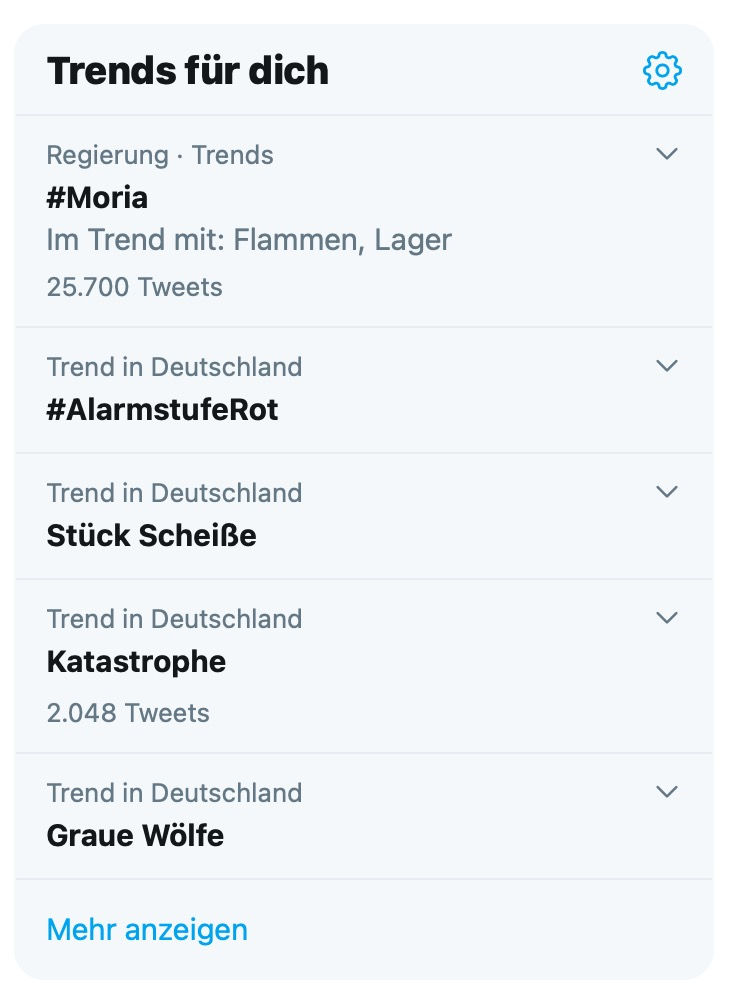
\includegraphics[width=0.28\textwidth]{images/twitter_trends.jpg}
    \caption{The trending topics on twitter. Collected on September 9th, 2020, 8.28am}
    \label{fig:twitter_trends}
\end{wrapfigure}

One feature that was not sufficiently finished when the user tests became was a sort of \emph{trend analysis} using the collected tweets. The plan was to show users trending topics for each day in the data set. Due to Twitter's limitations in their API, it was not possible to retrieve the daily trends that Twitter already collects and shows. 
To overcome this limitation, collocations were calculated for the tweet texts of each day. Collocations are \say{a lexical phenomenon} that \say{cover word pairs and phrases that are commonly used in language} (\cite[2]{mckeown2000collocations}), which means that they are word pairs that encounter together more often than by pure chance. The idea was that by calculating collocations on the tweets of a day, those word pairs could be phrases that were talked about on this day. While for some days the results seemed promising, for most of the days the calculated word pairs did not give much information. While it is possible that tweaks on the algorithm which calculated the collocations could have yielded more informative results, these tweaks could not be implemented before the user tests started.

Another feature that was planned, but not included, were tooltips in both visualizations. The tooltips were planned to include details, like the date and the specific value of the sentiment when hovering over a point on the line chart. While tooltips are generally possible in D3 for different chart types, there was no time left to properly implement them. For the bar chart, a work-around was used: Title-attributes were added to the div-containers that create the bars using the code seen in figure \ref{code:details_title}. By hovering over the bars, this title attribute is shown, which contained the date, the total number of tweets, the number of tweets containing the search word, and the percentage of tweets containing the search word. As the line chart is not built using divs per day, but rather from a single SVG element, this workaround could not be used in the chart showing the development of the sentiment over time.

\begin{figure}[h!]
    \begin{verbatim}
        svg.append("rect:title")
        .text(
        d =>
        `${formatTime(d.date)} | ${d.query_count} von ${
            d.total_count
        } Tweets (${(d.percentage * 100).toFixed(1)} %)`
    );
    \end{verbatim}
    \caption{The code that adds the date, the number of words containing the search word, the total number of tweets, and the percentage of words containing the search word to the bin of every day.}
    \label{code:details_title}
\end{figure}

As shown in chapter \ref{sec:fetchedData}, the country of origin for every tweet was collected. With this, a visualization could have shown differences in tweeting behavior between different countries. A theoretical example would be the questions if tweets about a Covid-19 vaccine that come from Russia are more positive than tweets about a vaccine that were tweeted from other countries. However, out of the 2.5 million tweets collected, only around 20,000 contained the origin country. Because of this small amount of data, this feature was not implemented.

Another data point that was collected, but ultimately not used, was the verification status of the tweets' authors. The initial plan was to offer users an option to compare tweets from verified and unverified sources. The plan was to include a toggle that breaks up the existing bar chart and line chart with another dimension \emph{is\_verified}. This would have added a lot of complexity to the visualizations for the users. Because the focus of this work is on visualizations that can be easily read and understand by laymen, this feature was eventually scrapped before the user tests.

\subsection{Testing the dashboard}
The user tests of the dashboard were testing two things: how users explore the dataset using the dashboard, and how easily they can read the two visualizations. For this, a guide for a semi-structured interview was prepared (see Appendix TODO). %TODO: Die Semi-Structured Quelle hierher packen!
The test consisted of two parts. After a brief introduction to the topic of this master thesis and a quick overview over the dataset, participants got around five minutes to explore the dashboard however they wanted. During this time, they were already asked to think aloud.

After this phase of free exploration, the participants were presented with four tasks in total with increasing difficulty. These tasks were designed to check the participants' ability to properly read the data visualizations. Again, participants were asked to think aloud while solving the tasks.
\begin{itemize}
    \item Task 1 was to find out on which day most tweets were sent. This task can be solved by finding the longest bar in the bar chart. It didn't matter which word was entered as the search word, as participants were asked to find the highest \emph{total} number of tweets, which can always be seen in blue. However, participants should toggle both neutral tweets and retweets to show up in the data set. After finding the highest bar, participants could hover over it to find the date in the tooltip.
    \item Task 2 was to find out on which day the most tweets were sent about Dr. Drosten. This search term was used to see if the participants could figure out that the search is, in fact, a filter. Only very little results were found typing in \say{Dr. Drosten}. Participants had to search for \say{Drosten} instead. This task also aimed to find out whether participants understand the difference between the day with the absolute highest number of tweets and with the relative highest number, compared to the total number of tweets that day.
    \item Task 3 was to find out how the sentiment about Dr. Drosten was when the neutral tweets were filtered out. This task tested two things: first if the quick filters were recognized as such, and if their job was clear. Then, the participants' ability and willingness to discuss ambiguous results was tested. The sentiments of tweets about Dr. Drosten changed significantly over time, with various peaks in both positive and negative sentiment as seen in figure \ref{fig:sentiment_drosten_noneutral}. Thus, there was no definite answer to the question. Participants had to read the data carefully and interpret it.
    \begin{figure}[h!tb]
        \fbox{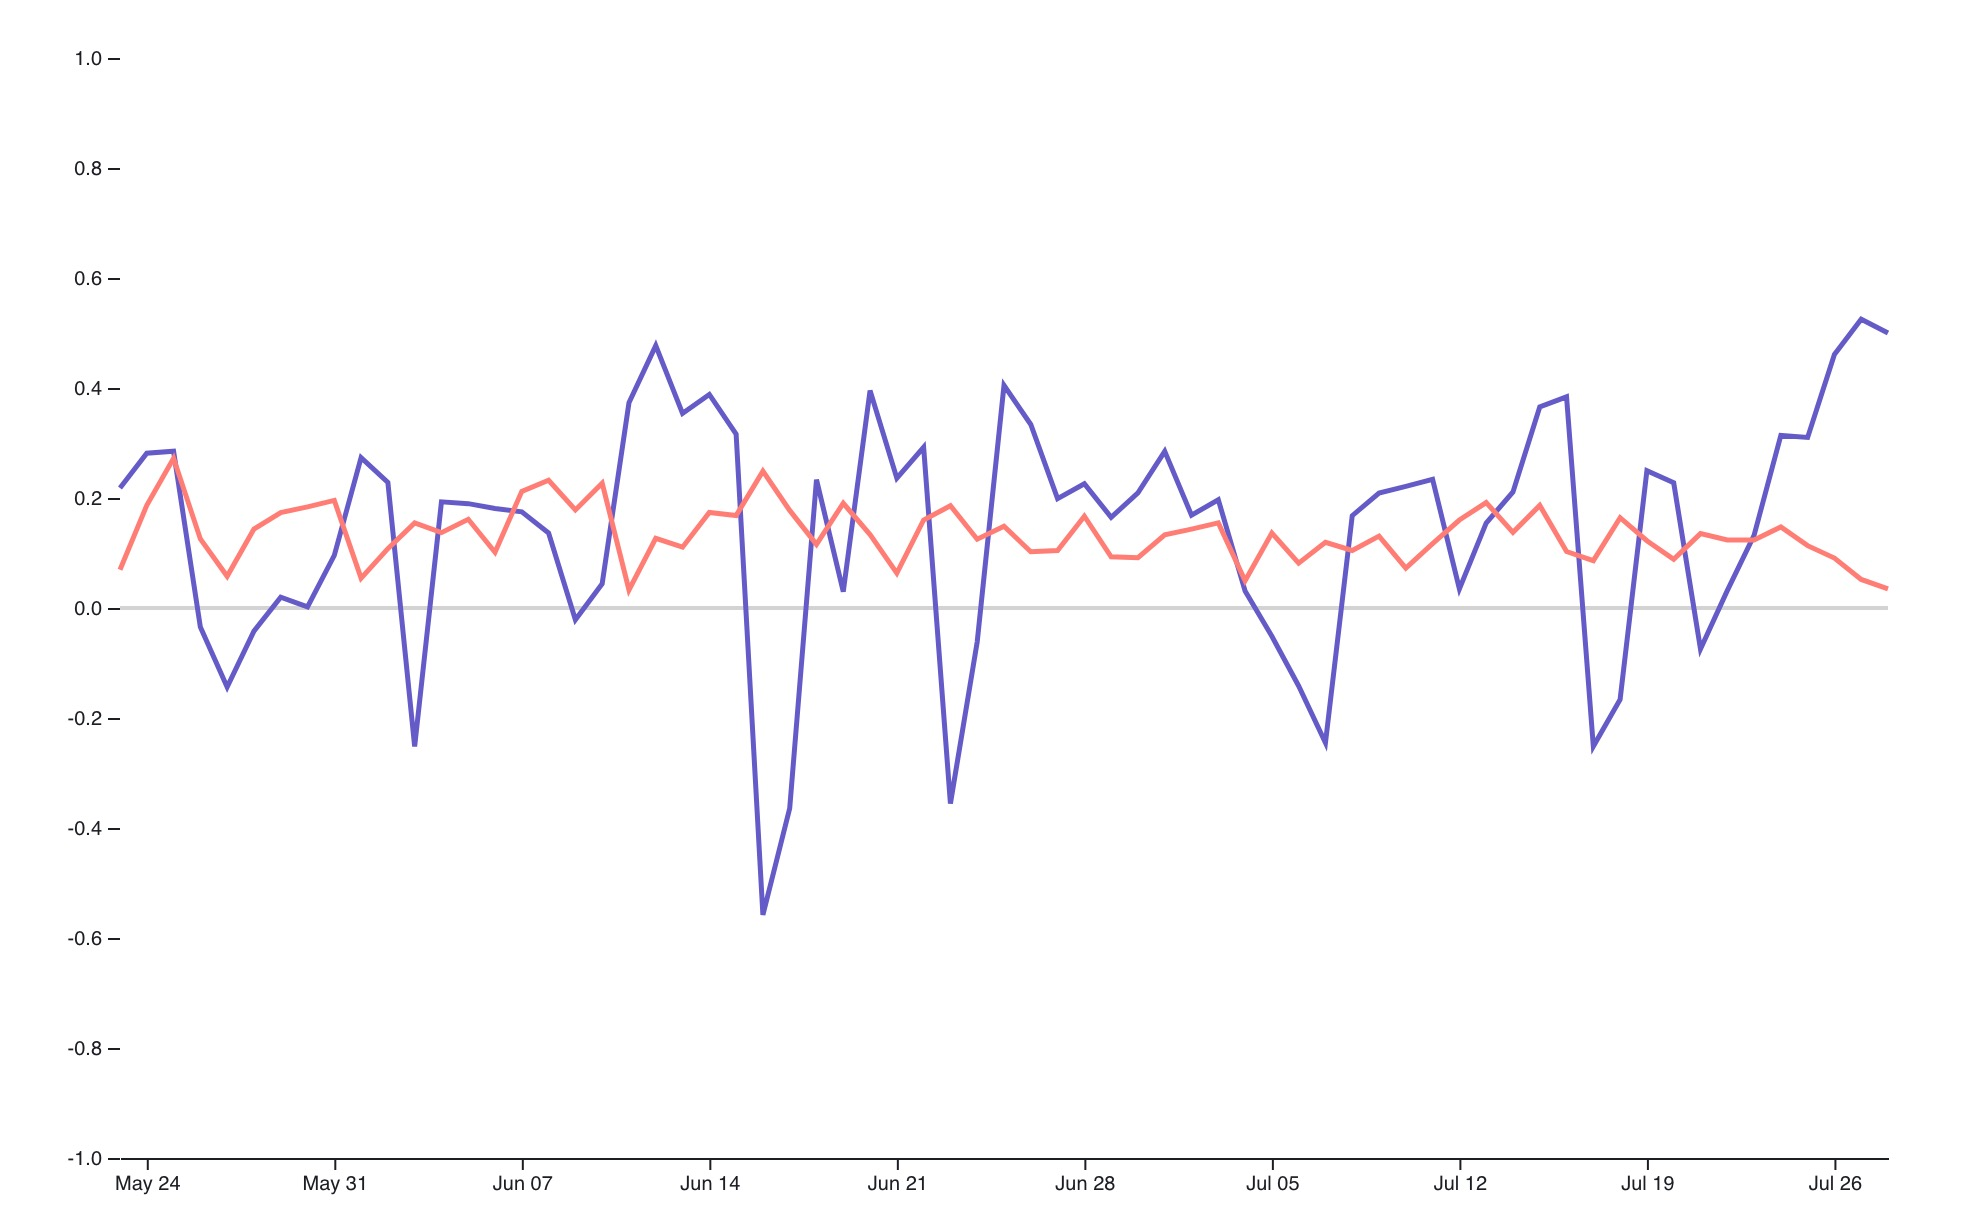
\includegraphics[width=\linewidth]{images/sentiment_drosten_noneutral.jpg}}
        \caption{The daily average sentiment of tweets containing the word \emph{Drosten}, without neutral tweets.}
        \label{fig:sentiment_drosten_noneutral}
    \end{figure}
    \item Task 4 was another task to test the participants' ability and willingness to discuss their findings. %TODO: why should they be able to discuss findings? It's important from a data literacy-perspective.
    For this final task, participants were asked to find out how retweets influence the overall sentiment of the German twitter discussion about covid-19. To solve this task, participants had to observe the influence the retweet-filter had on the sentiment graph and discuss this change. As in task 3, there is no definite right or wrong answer.
\end{itemize}

After the participants had completed the four tasks, a retrospective interview was conducted. The retrospective interview asked participants about their experience working with the tool and solving the tasks. Questions that arose during testing were also asked in the retrospective interview instead of during testing itself. Participants were also asked to report whether they had any questions in mind that they thought they should be able to answer using the dashboard.

Due to the ongoing Covid-19 pandemic, the interviews were conducted with the online video conference system Zoom\footnote{https://zoom.us}, rather than in person. Conducting the interview using Zoom had both advantages and disadvantages. On the one hand, Zoom allowed easy recording of both the audio, the screen, and the participants' webcam, which made transcribing easier. Participants could also take part in the study from their own home, rather than having to travel to a prepared test room. This made it possible to ask participants who did not live in Aachen to take part in the interviews.
On the other hand, even though Zoom does not require a lot of setup, this meant that people without access to their own internet-capable device could not participate in the study. Also, less tech-savvy people could have been hindered from participating in the study because they didn't want to or didn't know how to install Zoom and join the video conference.

The recorded zoom meetings were later transcribed to a reading version. After this, the transcriptions were coded based on Mayring's approach to qualitative content analysis (\cite{mayring2010qualitative}). For this, a deductive approach was used. Categories were derived from the material and sorted into two primary categories: \say{Motivationsfaktoren} (\emph{motivational factors}) and \say{Hemmfaktoren} (\emph{hindering factors}), based on whether the finding motivated the participants to use the tool or hindered their exploration. The code book, including anchor examples, will be discussed in the results section. 


\clearpage
\section{Results}
This Section describes the results of the interview study. First, a brief overview of the sample will be given. Then, the findings will be discussed, separated by motivational factors and factors that hindered the participants from effectively using and interpreting the charts. The final category system of the study is shown in \textbf{Figure \ref{fig:category_system}}.

\begin{figure}[htb!]
    \centering
    \fbox{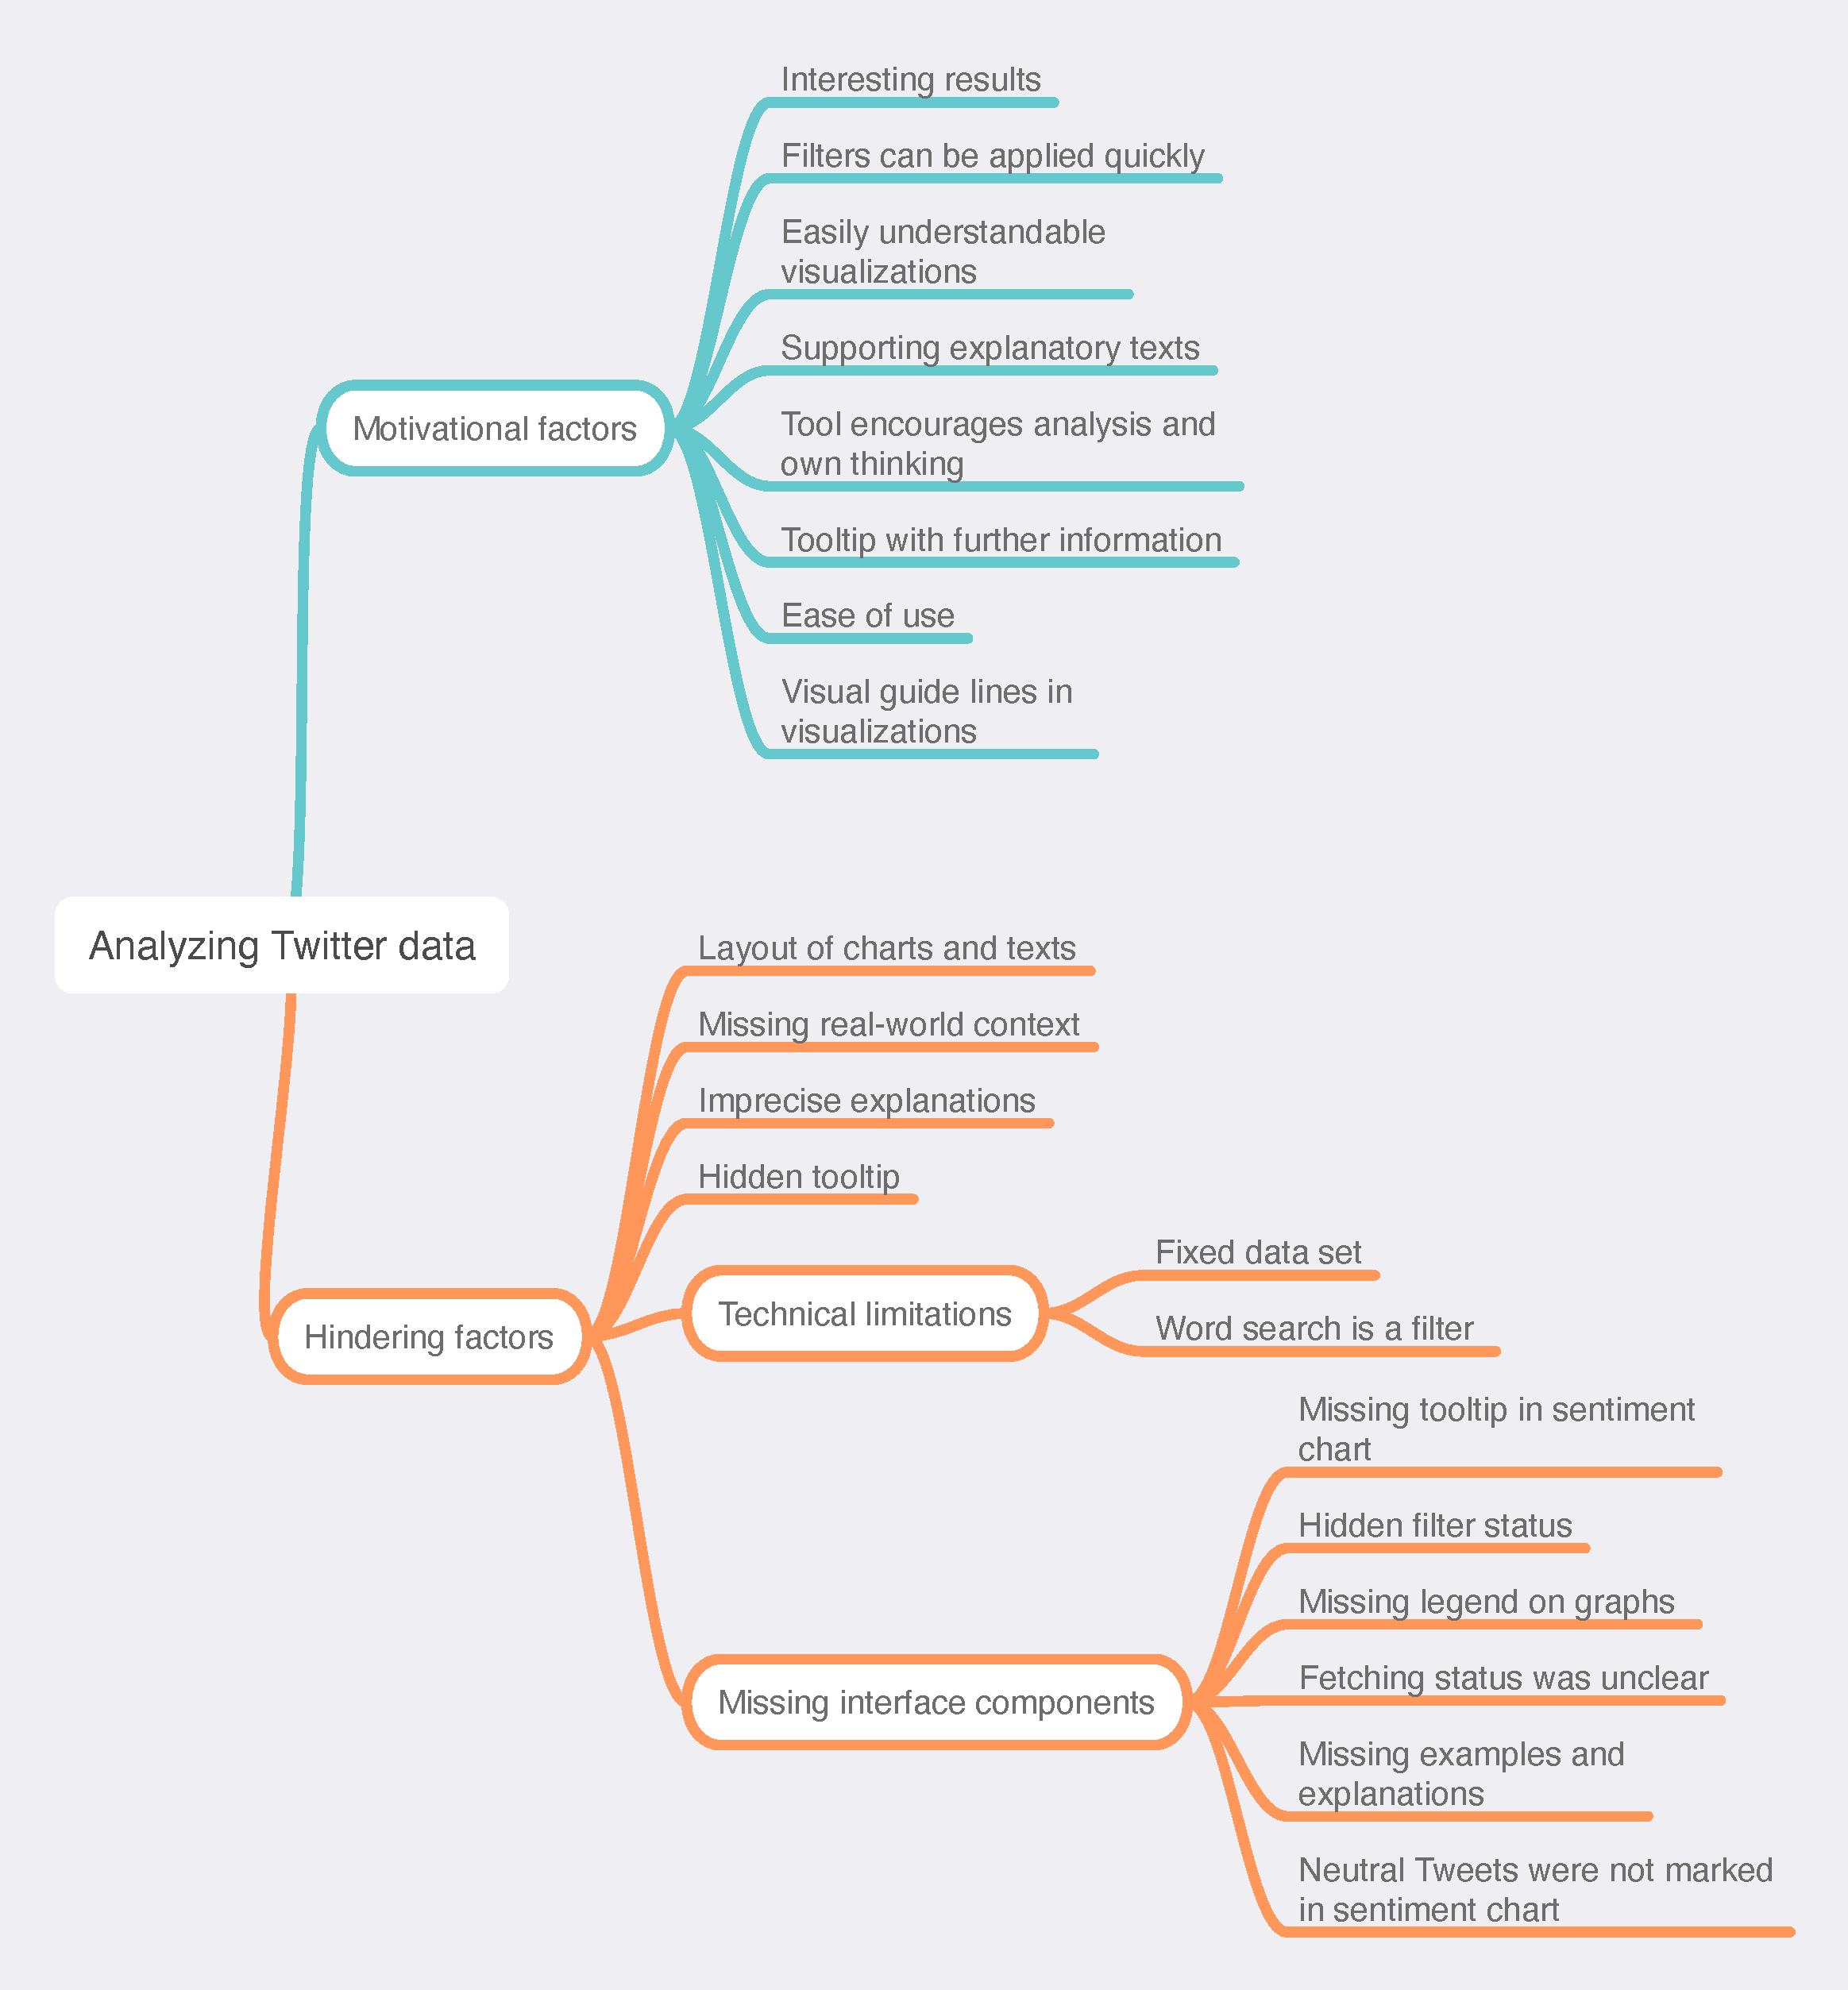
\includegraphics[width=\linewidth]{images/category_system.pdf}}
    \caption{The final category system.}
    \label{fig:category_system}
\end{figure}

\subsection{Sample description}
For the qualitative user study, six participants between the age of 23 and 26 were recruited. The study was limited to six participants because studies have shown that five to six user tests already uncover around 80\% of usability problems (\cite{10.1145/169059.169166}).

%TODO: grafische Aufbereitung der Ergebnisse des Screening-Fragebogens?

3 participants identify as male, 3 participants as female. The participants were chosen because they have little to no knowledge of Big Data and data visualization. This qualifies them as \emph{laymen}, the target group of this study.

Participants were asked to rate their interaction levels with twitter on a 6-point Likert scale from 1–never to 6–daily.

Twitter usage varied between the participants. 3 of them browse content on Twitter daily, 2 persons at least a few times a week. 1 participant never reads content on Twitter itself. All of the participants see twitter content at least sometimes on other web platforms. 5 participants rarely or never interact with content on Twitter, like using the like- or retweet button. The participants rarely post content on Twitter themselves.

\subsection{Motivational factors}
Motivational factors were factors that motivated participants to use the dashboard, explore the data set, and analyze the results. 9 motivational factors were identified in total which will be described in the following, along with anchor examples.

\subsubsection*{Interesting results}
Participants reported that they found the results they gathered from the visualizations interesting. One example is a participant who found it interesting that retweets make up most of the activity on Twitter:

\begin{quote}
    Aber schon spannend eigentlich, dass alles... also viele hauptsächlich Retweets sind und nicht eigene Tweets. (m23, l. 18)
\end{quote}

Others found the impact of retweets on the overall sentiment interesting:

\begin{quote}
    Ich fands sehr interessant zu sehen, wie so Retweets die Stimmung beeinflussen. (w25, l. 80)
\end{quote}

Participants also expressed that they liked to have the ability to see how a certain topic was discussed by the German Twitter-sphere:

\begin{quote}
    Aber ja, das ist schon interessant da mal nen Begriff reinzutippen und zu gucken, was passiert. (m24, l. 82)
\end{quote}

Some participants said that it was nice to see their own gut-feeling being backed by data:

\begin{quote}
    Ich finds sehr interessant zu sehen, wie so Retweets die Stimmung beeinflussen. Weil wenn man selbst Twitter benutzt merkt man halt auch selbst [...] dass mich persönlich das aufregt. Und das ist eigentlich sehr interessant gewesen zu sehen, dass das nicht nur mein Empfinden ist, sondern dass sich das generell in Twitter wiederfindet. Dass die Stimmung durch immer-wiederholen des gleichen Themas beeinflusst wird. (w25, l. 80)
\end{quote}

\subsubsection*{Filters can be applied quickly}
During testing, all participants used the toggles to show and hide retweets and neutral tweets multiple times in a row. This was likely done to compare the impact of retweets and neutral tweets on the data set.

\begin{quote}
    B: Und jetzt kann ich ja mal gucken wie sich das ändert, wenn ich die Retweets ausblende

    Screen: blendet die Retweets wiederholt aus und wieder ein (w26a, ll. 73-74)
\end{quote}

This behavior occured both during the free exploration and the task-solving phase of the interview.

\subsubsection*{Easily understandable visualizations}
Especially the bar chart which showed the tweet volume per day seemed to be easy to read for participants. This led to a quicker understanding of the data set and made it easier for participants to verify their assumptions. This participant, for example, wanted to see if a real-life event she knew of was reflected in the data set during free exploration:

\begin{quote}
    B: Ich probier es mal mit "Stuttgart", denn da gab es ja glaub ich eine der ersten dieser Hygiene-Demos
    
    Screen: gelbe Balken werden zwischen dem 21. und dem 24. Juni sichtbar
    
    B: Ah ja interessant, dann war diese Demo bestimmt am 21. Juni. Interessant. (w26b, ll. 6-8)
\end{quote}

Another participant explicitly said that both visualizations were easily understandable, even without further explanation:

\begin{quote}
    Und die Beschriftung der Achsen war auch so eindeutig, dass man... wahrscheinlich hätte ich da nicht einmal den Infotext gebraucht und die Grafiken hätten gereicht. (m26, l. 83)
\end{quote}

\subsubsection*{Supporting explanatory texts}
Participants reported that the explanatory texts that accompanied the visualizations were helpful. They aided them both in the exploration phase:

\begin{quote}
    Ich hab mich gerade kurz gefragt, was neutrale Tweets sind, aber hier unten steht ja die Erklärung dazu. (m26, l. 22)
\end{quote}

as well as while solving the tasks:

\begin{quote}
    I: Wie leicht ist es dir gefallen, die Aufgaben zu beantworten?

    B: Also ich würde sagen ziemlich leicht [...] Mit den Erklärungen fand ich die schon gut zu lösen. (w26b, ll. 68-69)
\end{quote}

\subsubsection*{Tool encourages analysis and own thinking}
Another point that participants liked was that the visualizations encouraged them to think about the meaning for themselves. One participant expressed joy that the interactive visualizations helped her answering questions she had on her own:

\begin{quote}
    Ne es gab ja so unendlich viele Corona-Visualisierungen immer. Und ich find das ganz cool, dass man hier sehr offen sich das anschauen kann. Weil sonst geben so Visualisierungen ja ziemlich genau vor, was man überhaupt sehen kann. (w26b, l. 63)
\end{quote}

Another participant liked that the tasks asked him to reflect on what he could read from the visualizations:

\begin{quote}
    Ja gerade jetzt die letzte Aufgabe war ja sehr interessant, fand ich. Das mal so zu sehen, dass das... ne also wenn man mal so drüber nachdenkt, den Effekt dann auch ein bisschen zu verstehen. (m24, l. 82)
\end{quote}

\subsubsection*{Tooltip with further information}
As previously discussed, the tooltip could only be realized in the graph that showed the tweet volume over time. This tooltip helped participants to explore the data set more efficiently:

\begin{quote}
    Screen: Hovert mit dem Mauszeiger über den längsten Balken
    B: Oh, gibt's hier... ne, doch, am 16.6. Ich hatte das eben gar nicht entdeckt, dass es nen Tooltip gibt, wenn man drüber hovert. Sonst hätte ich jetzt hier noch angefangen, die Tage abzuzählen. (m24, ll. 45-47)
\end{quote}

\subsubsection*{Ease of use}
This category contains statements from the participants where they expressed the ease of use of the visualizations. One participant said that she knew where to find which function after she saw the different parts of the interface once:

\begin{quote}
    Ich finde das sehr übersichtlich und eigentlich auch, wenn man sich das einmal angeschaut hat und einmal was wo find ich was, wo kann ich welche Daten aus- und wieder einblenden, schnell und gut benutzbar. Auch wenn man eigentlich nicht so ein Computer-Spezialist ist kann man doch sehr gut damit arbeiten. (w25, l. 78)
\end{quote}

Another participant said she was able to learn more about the way Twitter works in the prototype than on Twitter itself because the tool was easy to use:

\begin{quote}
    Aber prinzipiell ist das ziemlich cool und auch intuitiv. Also man kann ja selbst über diese Twittersuche sich relativ viele Daten selbst ziehen, aber das würdest du ja nicht machen wenn du da nicht selber so direkt mit rumspielen kannst. (w26b, l. 63)
\end{quote}

\subsubsection*{Guide lines in visualization}
Some participants voiced the usefulness of the guideline marking the 0-line in the line graph showing the sentiment (see \textbf{Figure \ref{fig:sentiment_drosten_noneutral}):}

\begin{quote}
    Ich würde sagen, also die Linie bewegt sich schon im Durchschnitt oberhalb des 0-Wertes hier, aber hier an manchen Tagen reißt sie deutlich nach unten ein. (w26a, l. 66)
\end{quote}

\clearpage
\subsection{Hindering factors}
Hindering factors are factors that hindered the participants in their usage of the tool in one way or another. These factors will be further examined and explained in the following Section.

\subsubsection*{Hidden filter status}
Participants had trouble recognizing that the search word had an impact on both graphs.

\begin{quote}
    Achso, das gesuchte Wort ist immer noch Covid hier in dem Graph, oder? Ah, okay. (m23, l. 20)
\end{quote}

Other participants were unsure whether the retweet and neutral tweet filters which were situated between the two visualizations had, in fact, an influence on the second visualization as well.

\begin{quote}
    Screen: Blendet die neutralen Tweets aus und scrollt zum Sentiment-Graph

    B: Eeehm... Moment, hat das hier nen Einfluss drauf?

    Screen: Togglet die neutralen Tweets nochmal an und aus

    B: Ah ja, hat es. (m24, ll. 58-61)
\end{quote}

Participants also reported that they forgot about the status of the filters while they were analyzing the visualizations:

\begin{quote}
    Und dann achtet man halt nicht auf solche Häkchen, die man irgendwie setzen kann, die sich dann auf alles auswirken. (w26b, l. 63)
\end{quote}

One participant also said that having to constantly scroll up to the filter status hindered her to effectively solve the tasks:

\begin{quote}
    Also es war eher die Frage, wie interpretiere ich das jetzt, welche Aussage kann ich aus dem, was ich da sehe, treffen. Und dann immer gucken "hab ich die jetzt eingeblendet, hab ich die jetzt ausgeblendet?", also da musste ich schon nen Moment länger drüber nachdenken. (w26a, l. 89)
\end{quote}

\subsubsection*{Missing legend on graphs}
Legends are used in color-coded graphs so that users can map the used colors to their meaning. An example of this can be seen in \textbf{Figure \ref{fig:legend_example}}.

\begin{figure}[h!tb]
    \centering
    \fbox{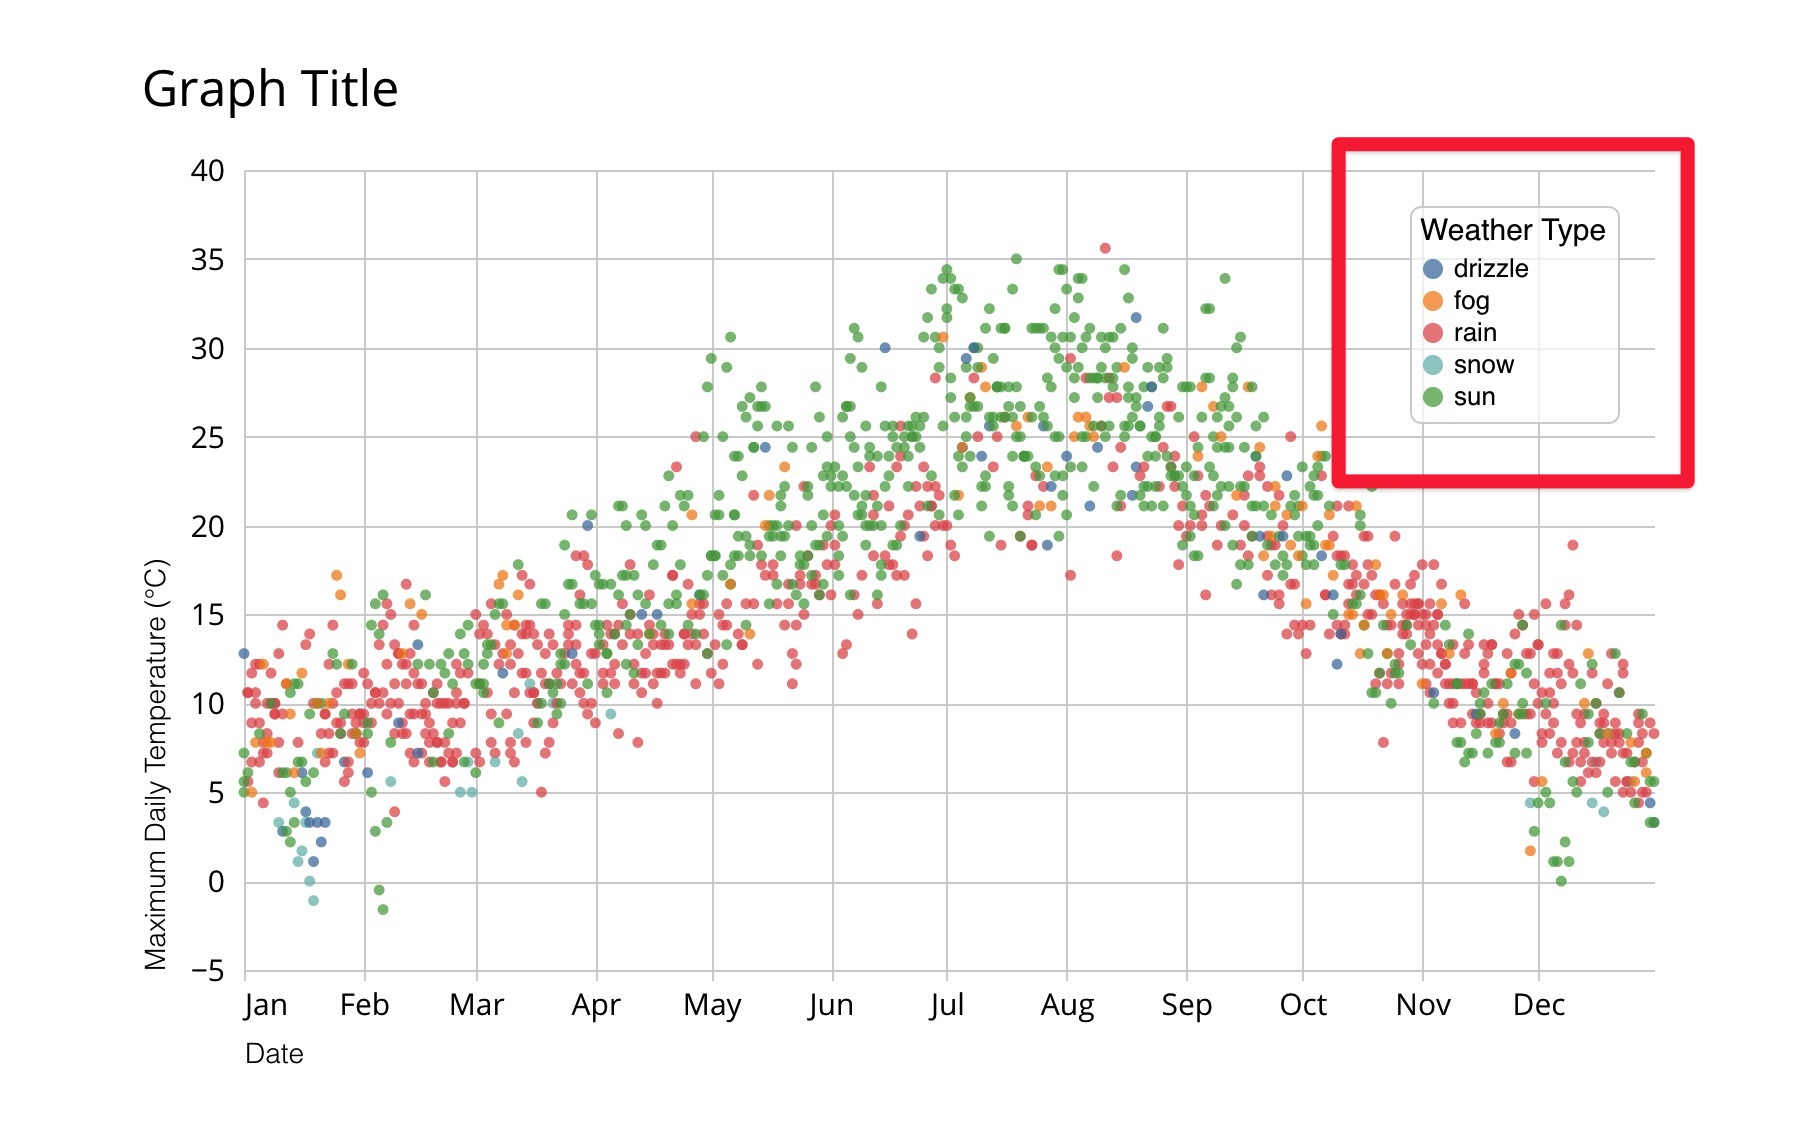
\includegraphics[width=0.7\linewidth]{images/legend_example.jpg}}
    \caption{Example of a legend showing which color corresponds to which data type. Screenshot from https://observablehq.com/@cahaber/cartesian-legend, highlight by the author.}
    \label{fig:legend_example}
\end{figure}

The prototype did not have such a legend. Instead, the meaning of the different colors was explained in explanatory texts. Due to Observable using a notebook structure, these texts could not be placed next to the chart and thus had to be placed either below or above it. In this prototype, the chart was followed by its explanation.%, as seen in figure \ref{fig:sentiment_nolegend}.

% TODO: will ich die Grafik drin lassen? Evtl. um Platz zu schinden.
% \begin{figure}[h!tb]
%     \fbox{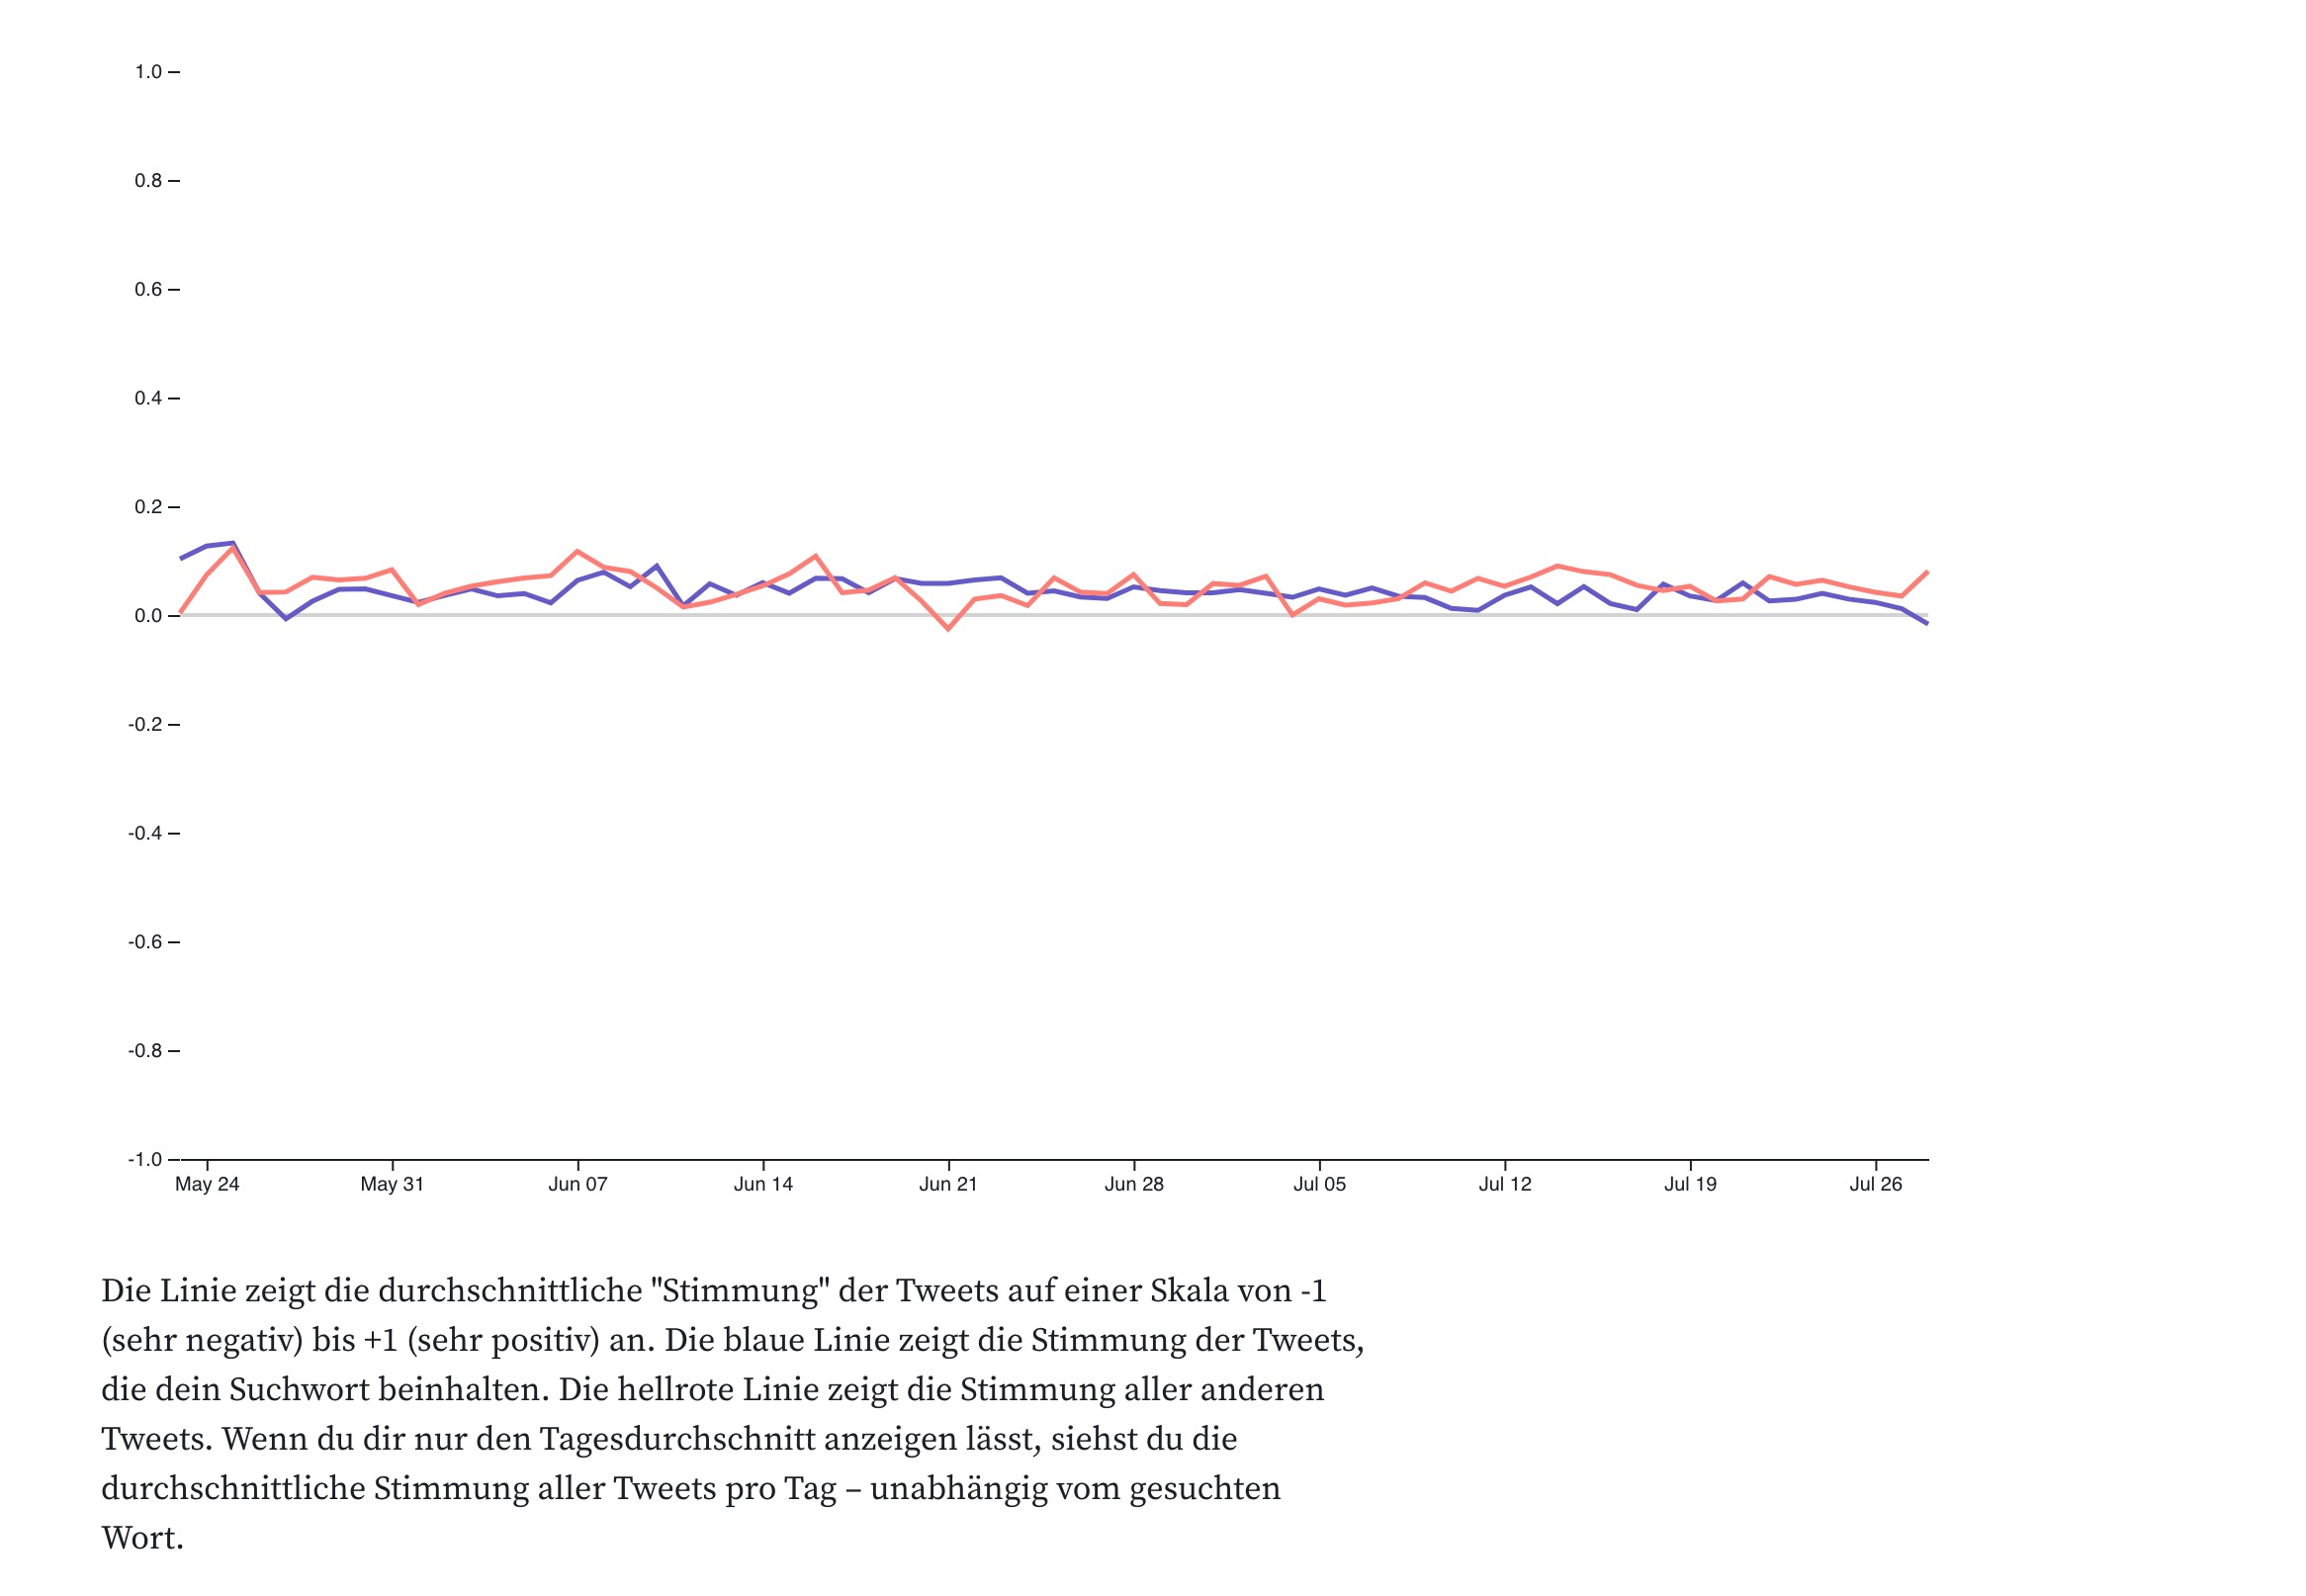
\includegraphics[width=\linewidth]{images/sentiment_nolegend.jpg}}
%     \caption{The sentiment chart with textual explanation of the colors below it}
%     \label{fig:sentiment_nolegend}
% \end{figure}

This resulted in several issues. One participant did not understand the meaning of the differently colored bars in the bar chart because she did not read the explanatory text thoroughly enough:

\begin{quote}
    B: Meine Frage ist jetzt nur, was bedeutet Orange und was bedeutet blau? 

    Screen: Scrollt etwas runter

    B: Da weiß ich aber nicht, ob das nachher noch kommt. Aber jetzt im ersten Moment hab ich nicht gesehen, was das bedeutet. (w25, ll. 8-10)
\end{quote}

The same participant had trouble recognizing the textually explained color in the sentiment chart.

\begin{quote}
    Screen: Scrollt zum Sentiment-Erklärtext runter

    B: Hä, rot? Ich seh gar keine hellrote Linie, sondern nur hier das Orange und blau.

    I: Ja, die orange Linie ist damit gemeint.

    B: Achso, okay. (w25, ll. 24-27)
\end{quote}

Another participant got confused by the textual explanation of the different parts of the chart. In this case, the word \say{blue} could have meant two different lines, one dark blue and one light blue.

\begin{quote}
    "Die Linie zeigt die durchschnittliche Stimmung..." Aber welche Linie ist denn jetzt DIE Linie? Dann gibt es eine blaue und eine hellblaue. (m24, l. 65)
\end{quote}

\subsubsection*{Layout of charts and texts}
This category contains problems that arose during testing that stem from the layout of charts and texts. One participant did not see the explanatory text for the sentiment graph, as it was below the graph itself:

\begin{quote}
    B: Okay, ich glaub ich hab noch nicht ganz verstanden, was mir der Graph sagen will. Also, Sentiment ist quasi die Wertung?

    I: weiter unten steht auch noch mehr Erklärtext dazu.

    B: Okay. Aaah okay, das ist der Text hier unten (m23, ll. 22-24)
\end{quote}

Another participant seemed to be confused by the sentiment chart. After he found the explanatory text below the chart, he could continue with the task.

\begin{quote}
    Screen: Scrollt wieder zum Sentiment-Graphen runter
    
    B: Ach aber auch hier kein besonders überraschendes Sentiment. Warte, was... was tut denn hier die blaue?

    Screen: Fährt mit dem Cursor über den Erklärtext unter dem Graphen
    
    B: Ah, okay. Joar, okay. Dann... vielleicht doch eher. (m24, ll. 28-31) 
\end{quote}

One participant explicitly stated that he would have preferred to have the explanation texts \emph{above} the charts.

\begin{quote}
    Ich glaub das einzige, was ich gemacht hätte, wäre, den Infotext über die Grafik zu packen. Das wär für mich praktischer gewesen, weil dann lese ich erst, was ich sehe, und sehe dann erst die Grafik. Wobei ich jetzt gerade auch nen relativ kleinen Bildschirm habe. (m26, l. 75)
\end{quote}

However, one participant who studies to become a teacher said that she liked the layout from a pedagogical perspective.

\begin{quote}
    I: Das heißt, für deinen Lesefluss und das Verständnis wäre es besser gewesen, wenn du den Erklärtext über der Darstellung hast, die erklärt wird?

    B: Das ist ne gute Frage, also ich glaube aus einer verständnistheoretischen Perspektive ist es wahrscheinlich schlauer, wenn man sich erst die Frage stellt, bisschen irritiert ist und dann die Antwort findet und dann das versteht. Wenn man es erst liest und nicht genau weiß, worauf sich das jetzt bezieht, muss man den Text im Zweifelsfall zwei Mal lesen. Weil dann liest du das halt, denkst "hä?", dann schaust du dir das an und merkst dann, dass du Informationen dazu bekommen hast. Und dann liest du dir das nochmal durch. (w26a, ll. 80-81)
\end{quote}

\subsubsection*{Word search is a filter}
This category contains statements in which the participants stumbled over the limitations of the word filter. The word filter filters for exact matches of the entered term in the database. This is different to search engines like Google or DuckDuckGo: These engines use a so-called \emph{fuzzy search}, which means that results do not only contain the exact search term, but also similar terms.

One participant entered a too specific keyword, but could quickly recover from this:

\begin{quote}
    Screen: Gibt "Dr. Drosten" in den Suchfilter ein

    B: Dann würd ich eben erst mal Dr. Drosten in diese Suchleiste hier oben eingeben

    Screen: wenige Ergebnisse werden gezeigt

    B: Wobei vielleicht geb ich besser nur "Drosten" ein weil den Doktor... filtern die Leute ja wahrscheinlich raus. (w26b, ll. 37-40)
\end{quote}

Another participant made a spelling mistake when filtering for a word which she did not recognize until she was made aware of it:

\begin{quote}
    Screen: Gibt im Wortfilter "Tonnies" ein, es werden nur sehr wenige Ergebnisse angezeigt

    B: Hm, jetzt seh ich hier gar nix

    I: Du hast Tönnies falsch geschrieben. Mit O statt mit Ö.
    
    B: Aah, I see. 

    Screen: Gibt Tönnies ein

    B: Okay, und verändert sich jetzt was? Ah ja, okay!  (w26a, ll. 10-15)
\end{quote}

Without the author's intervention, this participant most likely would not have been able to recover from her mistake, thinking that \emph{Tönnies} did not appear in the set of collected tweets.

\subsubsection*{Missing real-world context}
While the participants were able to identify days with high activity for a specific topic, the dashboard did not offer more information about what happened on that day. Some participants said that they could have used this information to interpret the findings better.

\begin{quote}
    B: Ganz witzig, am 5. und am 19. Juli gibts hier so... wie nennt man das denn, kein Peak sondern das Gegenteil  eines Peaks wo es dann so krass runtergeht. Das wäre interessant zu wissen, was an diesen Tagen war, ob die Leute da wohl schlechter drauf waren in Bezug auf Corona.  (w26b, l. 18)
\end{quote}

\subsubsection*{Fetching status was unclear}
When the word filter is changed, new data is fetched from the database. This means that it takes about five seconds between typing in a new search word and the results for this word being displayed. Participants felt unsure about whether their input had already been processed or if they had to wait a bit longer, as the fetching status was not shown in the interface.

\begin{quote}
    B: Da geb ich oben in diesem Suchbalken was ein. Da geb ich jetzt Dr. Drosten ein

    Screen: Die Grafik verändert sich, zeigt aber nahezu keine Ergebnisse. 

    B: Und... drücke Enter? Hat sich jetzt schon was getan?

    I: Ja, hat es.

    B: Ach, das hab ich gar nicht gemerkt. (w25, ll. 36-40)
\end{quote}

\subsubsection*{Imprecise explanations}\label{sec:unprecise_explanations}
This category contains statements from participants where an explanation for certain elements was given, but the explanation was not satisfactory. This contains imprecise wording or missing further information.

\begin{quote}
    Sentiment ist noch so... ich weiß noch nicht so ganz, was das heißt. Also klar, was das irgendwie bedeuten soll, aber... wie sieht jetzt zum Beispiel ein positiver Tweet aus oder ein negativer. (m23, l. 73)
\end{quote}

\subsubsection*{Tooltip was not found}
This category contains passages where participants did not see the tooltip in the bar chart. As discussed before, the bar chart which shows the tweet volume has a tooltip, while the line chart showing the sentiment over time does not have one. Statements in this category were thus always connected to the bar chart.

One participant counted the bars while solving task 2 (finding the day where most tweets were sent about Dr. Drosten):

\begin{quote}
    B: Aha! Und dann würde ich behaupten... das ist der 24., 25., ich würde sagen das ist der 27. wobei das relativ close ist mit dem... 22., 23., 24. 

    Screen: Das Popup erscheint zwar, sie zählt die Tage trotzdem noch an der X-Achse ab (w26a, ll. 60-61)
\end{quote}

\subsubsection*{Missing examples and explanations}
Some participants stated that they would have liked further examples or explanations to deepen their understanding of the visualizations and the data they were based on. As opposed to subsection \ref{sec:unprecise_explanations}, these statements were not about the quality of existing explanations, but rather about pieces of information that were completely missing from the interface.

One participant said that a guide would have been helpful for him to analyze the data better. This could include a short explanation of how the algorithm works, as well as examples of specific tweets, their calculated sentiment, and why exactly this sentiment was calculated.

\begin{quote}
    Also... so was man beachten muss, wenn man mit nem Sentiment arbeitet. Und wie man die... also so ein bisschen ne Interpretierhilfe, glaube ich. (m23, l.. 75)
\end{quote}

Other participants said, for example, that they would have liked to get a better explanation of how the sentiment analysis worked (cf. w25, l. 17; m23, l. 73). Then again, one participant explicitly said that she does not think further information about the sentiment chart would help her understand it better:

\begin{quote}
    I: Hättest du dir da ne Erklärung zu gewünscht wie das klappt?

    B: Nö, nicht unbedingt. Das ist glaub ich so technisch, dass ich als nicht unbedingt Informatik-affiner Mensch das überhaupt verstanden hätte. Also da hätte ne Erklärung stehen können, aber ich glaube nicht, dass die mir geholfen hätte. Weil ich als Anwender denk hauptsächlich "Hauptsache es funktioniert" und ich weiß was ich machen kann, wenn es nicht funktioniert. Aber wie genau das Programm geschrieben ist muss ich als Anwender nicht unbedingt wissen. (w25, ll. 18-19)
\end{quote}



\subsubsection*{Missing tooltips for the sentiment graph}
After participants had found the tooltips for the bar chart, they expected to see tooltips for the line chart depicting the sentiment as well.

\begin{quote}
    B: Da sehe ich, dass das ziemlich schwankend war, dass zum Beispiel hier am... 

    Screen: hovert über die Spitzen des Line Charts

    B: der genaue Tag wird nicht angezeigt, wenn ich hierdrüber gehe. Aber es war auf jeden Fall zwischen dem 14. und 21. Juni (w25, ll. 56-58)
\end{quote}

\subsubsection*{Neutral tweets were not marked in the sentiment chart}
While the zero-baseline was marked in the sentiment chart, the area between -0.3 and +0.3 was not. While solving the tasks, participants looked for spikes in the sentiment that grew above 0.3 or below -0.3 for easier interpretation. The interface did not support this because the neutral area was not marked. Also, the aforementioned missing tooltips for the sentiment graph hindered some participants to effectively discuss their findings.

\begin{quote}
    Und wir sehen, dass wir hier periodische Ausschläge haben, positiv wie negativ. Uuund... wir sehen hier zumindest ein, zwei, drei, vier Spitzen, die negativ sind. Also ein Sentiment über -0,3 haben... wobei, dann sind die beiden hier vielleicht nicht mit dabei, die sind nicht über 0.3. (m26, l. 55)
\end{quote}

\subsubsection*{Fixed data set}
One participant said that she would have liked to have more data and to be able to scroll or scrub through different states of the public discussion about Covid-19.

\begin{quote}
    Kann ich da auch noch nach links weiterscrollen, dass es nicht erst im Mai losgeht sondern schon im März? Hm ne. (w26b, l. 6)
\end{quote}

Saying this, she hovered on the left edge of the visualization. 


\clearpage
\section{Discussion}
This section will discuss the findings from the interview study. For hindering factors that were found, a possible solution will be discussed. For motivational factors, ways to further improve these factors will be taken into consideration.

\subsection{Motivational factors}
During the coding process of the interviews, several factors that motivated participants to use the prototype were found. Here, these motivational factors that were found during testing are discussed. Possible ways to further strengthen these points in future developments of the tool are proposed in this section.

\subsubsection*{Easily understandable visualizations}
The participants said that the visualizations were easily understandable. Future development should keep in mind that the ability to quickly understand the visualizations motivated the participants to discuss the results further, rather than being preoccupied trying to understand what the visualization tries to show them.

To keep the visualizations easily readable, the paradigm \emph{one job per visualization} should be followed. The clear separation of concerns between the two visualizations seemed to support the participants when answering questions. If new visualizations should be added to the tool, this should be done in a separate chart, rather than by adding new elements to one of the existing charts.

The separation of the visualizations could be deepened even further by showing the different visualizations in different tabs. During the user tests, the participants rarely referred to the other visualization during interpretation.

\subsubsection*{Interesting results}
Participants said that the results are interesting and surprising, which according to \citeauthor{northMeasuringVisualizationInsight2006} is an indicator that they could gain insight. Future versions of the prototype could allow participants the easy exporting of specific results to share them with interested friends if they find results surprising or interesting. Participants also reported that the tool made them reflect their own beliefs of how social media works and how discussions unfold.

\subsubsection*{Supporting explanatory texts}
The explanatory texts helped the participants understanding the visualizations and the capabilities of the tool better. As already discussed in chapter \ref{sec:missingExamples}, these explanatory texts can be further improved, e.g., by adding examples and hints for analysis.

One thing that could be changed about the explanatory texts is their position. Due to the nature of Observable, which was used to build the prototype, explanatory texts were always visible and did not only show in context. One way to further improve the way the texts are presented is by visually hiding some of the texts in the interface. For this, texts should be divided into two kinds:
\begin{enumerate}
    \item Texts that are essential to understanding the visualizations
    \item Texts that offer additional help, insights, explanations, or inspiration for analyzing the data set
\end{enumerate}

Dividing texts into these two categories could result in a less cluttered interface. Important texts from the first category can be always shown, while texts that fall into the second category can be hidden, e.g., in tooltips or detail panes. Showing only necessary texts also means that the visualizations are front-and-center in the tool, attracting the users' attention. It would also eliminate the need to scroll a lot when accessing the tool from a laptop or tablet (cf. m26, l. 75). One example how these hints could be shown can be seen in figure \ref{fig:sentiment_tooltip_hint}.

\begin{figure}[htb]
    \centering
    \fbox{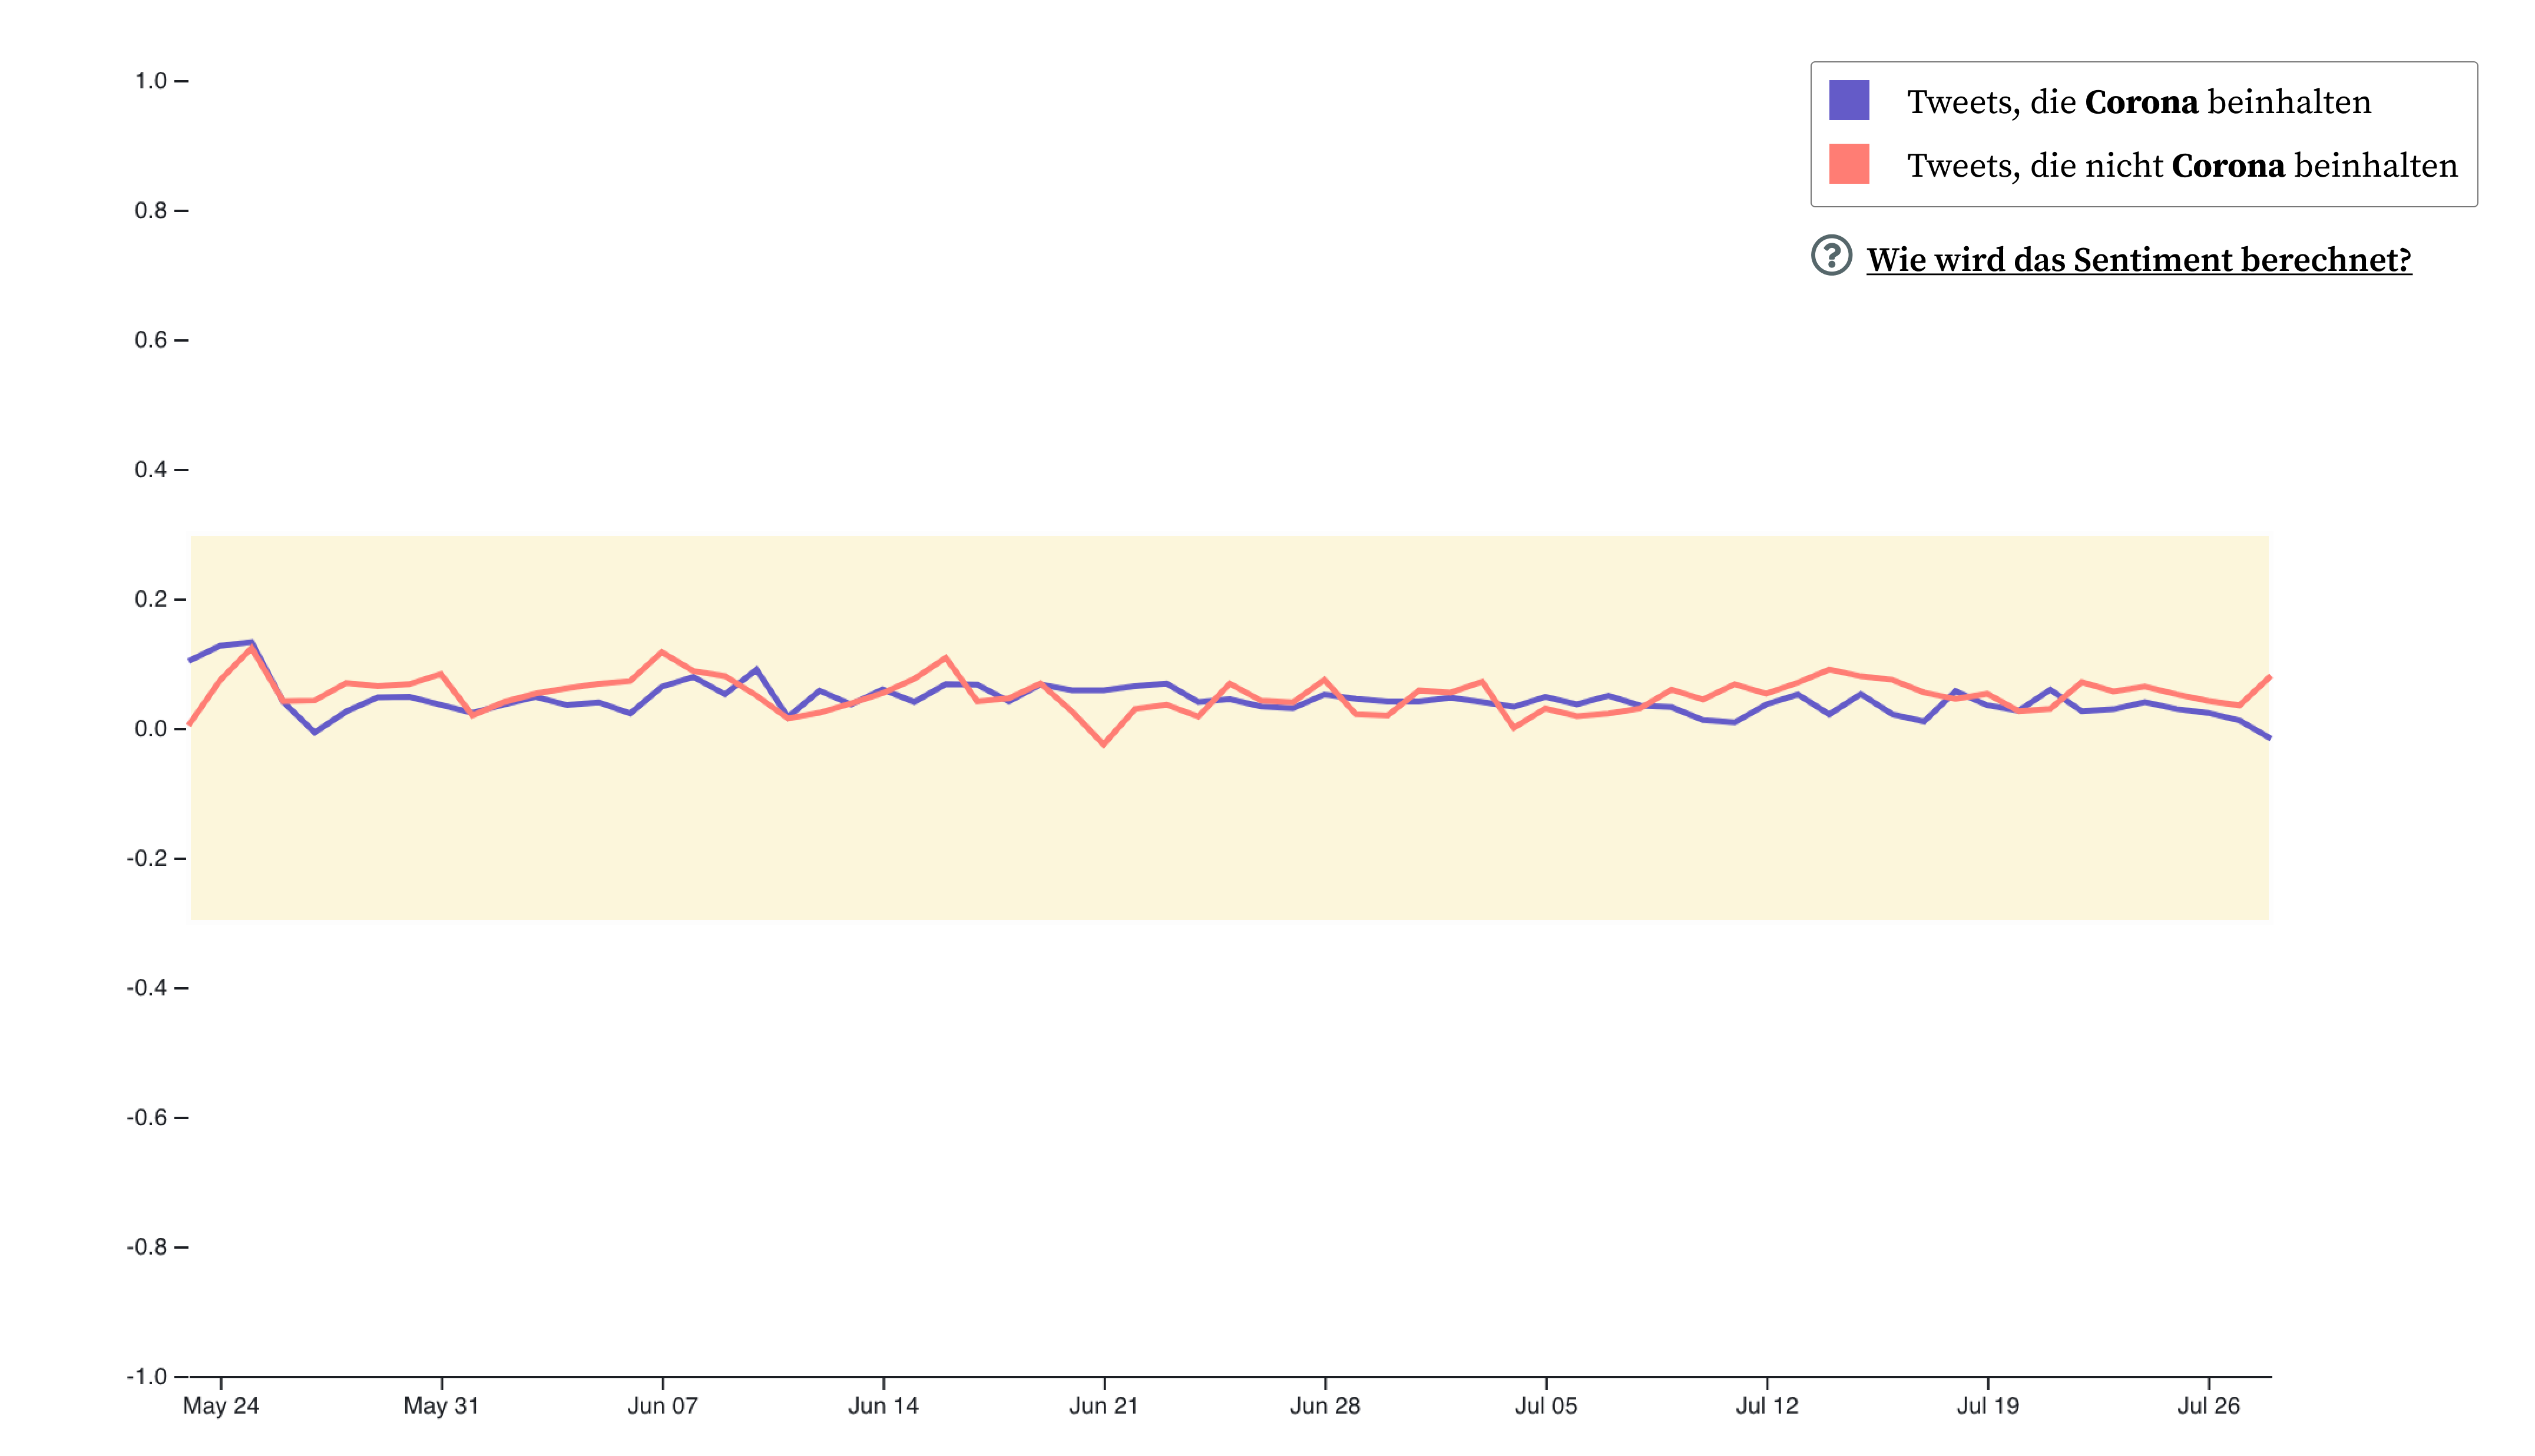
\includegraphics[width=0.98\linewidth]{images/sentiment_tooltip_hint.png}}
    \caption{A proposed tooltip target for additional explanations regarding the sentiment analysis.}
    \label{fig:sentiment_tooltip_hint}
\end{figure}

\subsubsection*{Filters can be applied quickly}
Except for the word filter, which had to fetch new data from the database, the filters could be applied quickly. This seemed to support how participants worked with the tool while solving the tasks during the interview as well as during the free exploration. This suggests that future development of the tool should focus on keeping the quick filters for toggling retweets and neutral tweets should keep this interaction quick instead of fetching new data every time one of these filters is toggled.

During user tests, the toggles were mostly used for a before-and-after view of the dataset, e.g., quickly toggling the retweets to visually compare the impact the retweets had on the tweet volume. This interaction could be further improved. One example could be to introduce a button that can be held down to turn all filters on or off. Holding down the button could show the 'original' data set without the retweet- or neutral tweet filters applied, letting go of the button shows the filters the users applied before again. A similar interaction can be found in image manipulation software like Apple Photos, where holding a button switches between the original photo and the manipulated version.

\subsubsection*{Tooltip with further information}
The tooltip that was shown in the volume chart helped participants finding answers to their questions. Future development could focus on making this tooltip more helpful. One important step for this would be to create a more visually appealing tooltip which contains styled information. The tooltip that was eventually used in this study could only handle single strings of unstyled text. However, text styling is one of the most efficient ways to structure information so that it can be easily digested. 

\subsection{Hindering factors: missing interface components}
Some of the problems that were mentioned can be solved by introducing additional interface components. The problems and their proposed solutions are discussed in this section.

\subsubsection*{Overview of currently set filters}
Multiple participants had trouble recognizing what data filters were applied for the current visualization. The idea that the filters can be changed on top of the notebook and will then influence the rest of the visualization does not seem to work, especially on smaller laptops, as this resulted in a lot of scrolling.

\begin{figure}[htbp]
    \fbox{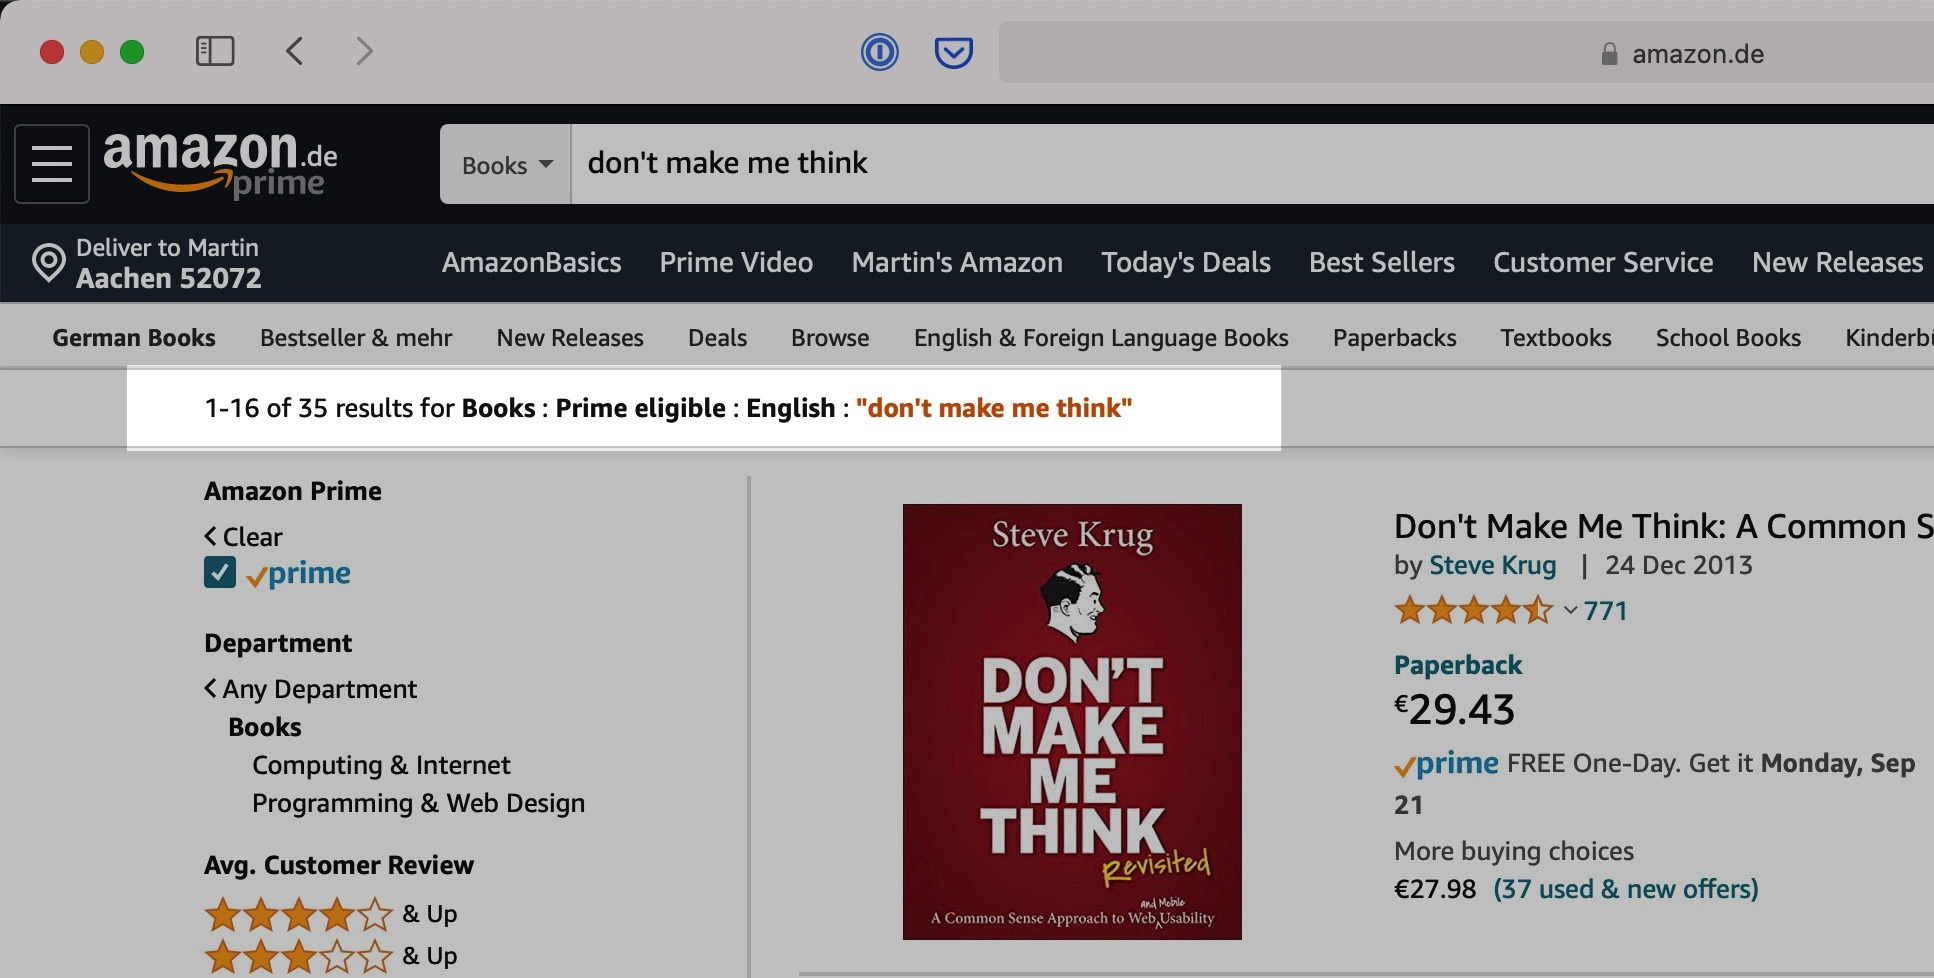
\includegraphics[width=\linewidth]{images/amazon_filters.jpg}}
    \caption{The Amazon search is filtered to English-language books which are eligible to prime-shipping, with the search input \emph{don't make me think}. Highlight by the author}
    \label{fig:amazon_filters}
\end{figure}

This means that the filter status should be visible directly next to the visualization. This way, participants would not need to search for the current filter status. Rather, the status would almost always be in view while interpreting the visualizations. There are two possible ways to show the filters near the visualizations:
\begin{enumerate}
    \item \textbf{Show a descriptive text above the visualization:} using a text to show the status of the filter could help participants to quickly understand what kind of data the visualization is showing at the moment. One example of this technique can be found on Amazon, as seen in \textbf{Figure \ref{fig:amazon_filters}}. This technique is especially useful when a lot of different filters can be applied.
    \item \textbf{Show the filter toggles right next to the visualization:} instead of showing the filter status as a text, showing the filters with the actual toggles would allow users to change the filters right next to the visualization.
\end{enumerate}

\begin{figure}[h!tbp]
    \fbox{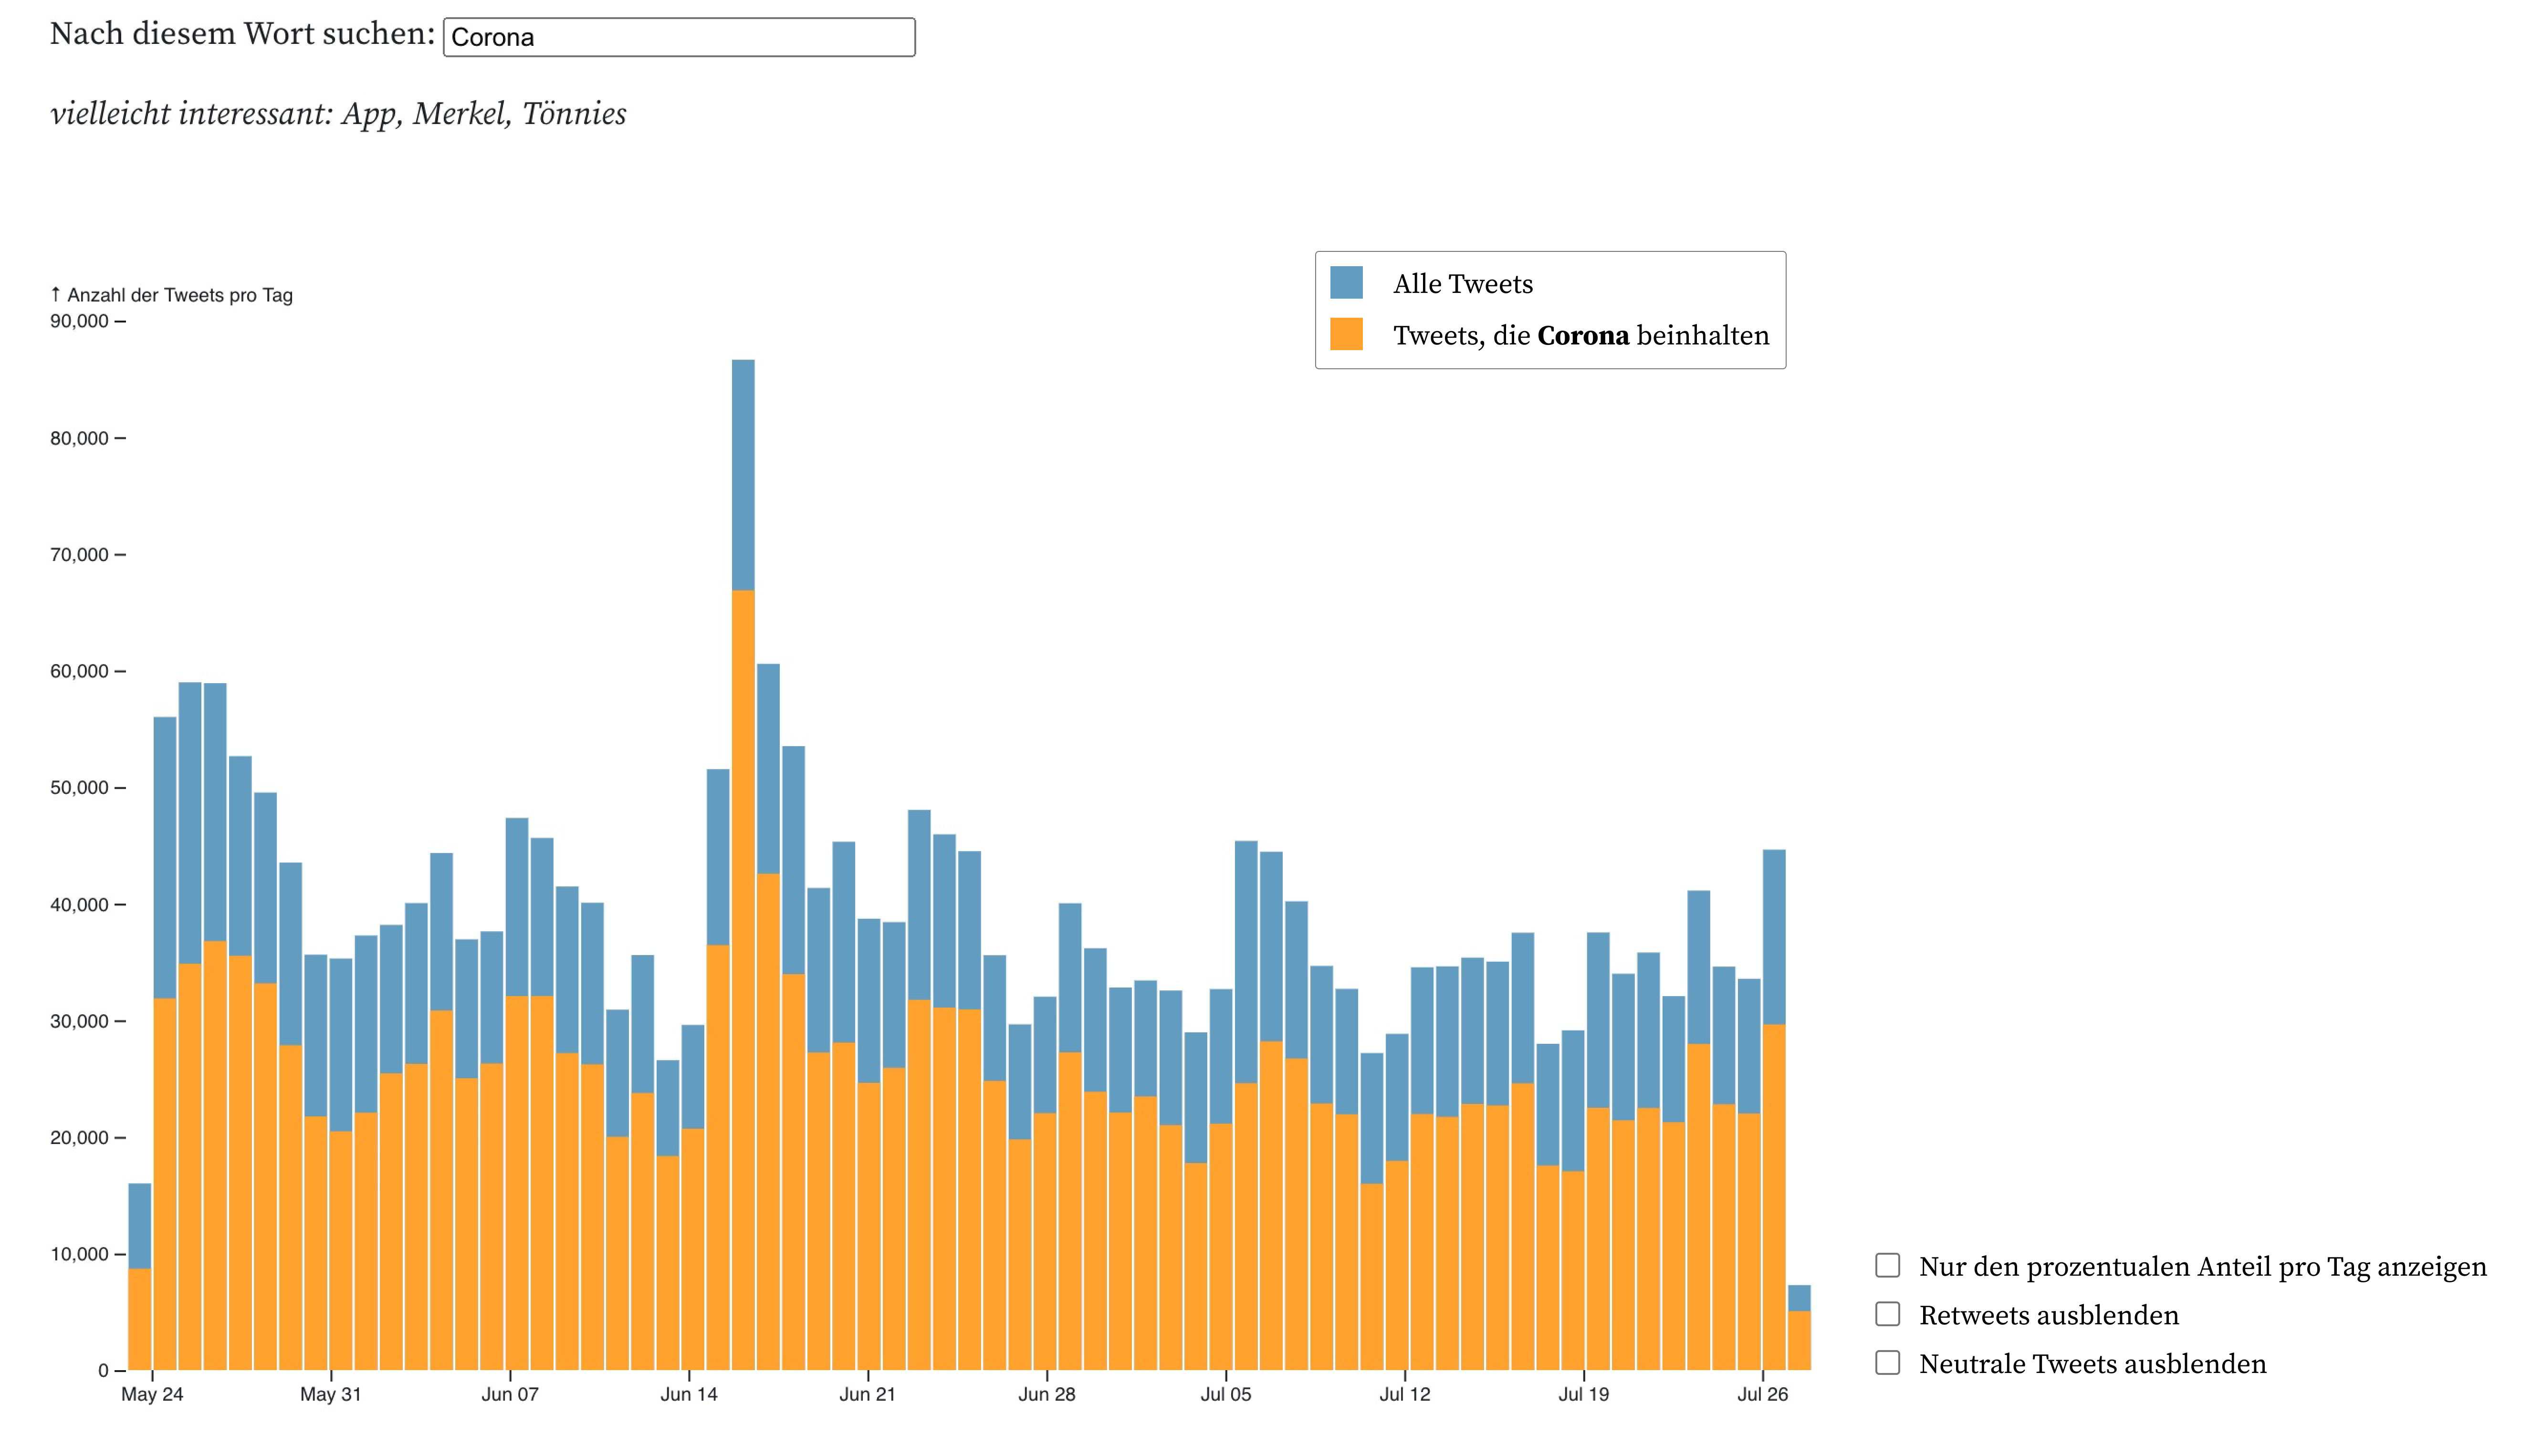
\includegraphics[width=\linewidth]{images/legend_and_filters.png}}
    \caption{Proposed layout of the tweet volume with a legend and filters directly next to the graph}
    \label{fig:legend_and_filters}
\end{figure}

Showing the filter toggles right next to the visualizations seems like a straightforward idea. However, this raises the question if the filters of the two visualizations should be linked or not, i.e., should the filter of the sentiment graph change as well when the filter of the volume graph is changed or not. To decide this, further studies should be conducted to see if the synchronicity of the data visualizations is helpful or not.

This study did not examine if it helps users to have a single filter context within several visualizations or not. During the exploration phase in the interview, however, the participants did not seem to switch a lot between examining the tweet volume and the sentiment chart. This could suggest that having a single filter applied to both visualizations is not a necessity. In this case, using two filter sets that are independent of each other could avoid user confusion as only explicit user actions influence the visualization.

\subsubsection*{Color legend}
Another missing interface component are colored legends. During user testing, several problems arose because of the missing legend. For one, the graphs were less self-contained. Users were forced to read the explanatory texts that accompanied the graphs to be able to understand what the different colors mean. Another problem with the textual explanation of colors was that different participants would have named the colors differently than the text did and were confused, e.g., when the text talked about a light-red line, but the participants only identified an orange one. A legend like the one shown in \textbf{Figure \ref{fig:legend_example}} could have helped to identify the colors more easily, as well as making the graph more self-explanatory.

\textbf{Figure \ref{fig:legend_and_filters}} shows a proposed addition to the tweet volume-graph. Implementing these changes makes the current filter status more obvious and lets users toggle the different filters without needing to scroll to the top of the notebook again. The legend with dynamic labeling, which includes the search term the user entered, makes the graph more self-contained.

The added legend could also help solve the layout problem that participants mentioned. With the explanatory texts no longer necessary to understand the graphs, the texts serve as an additional explanation and, as such, can remain below the graph itself.

\subsubsection*{Loading indicator}
Another component that was missing from the interface was an indicator that new data was fetched from the server. One possibility to show this fetching would be to show a small loading indicator next to the word filter. However, this position could hide the loading indicator, making it not noticeable enough. It would also not indicate that the visualization does not yet reflect the selected data set.

Another possibility would be to show in the visualizations themselves that new data is being fetched. As fetching takes about 5 seconds and the visualizations have not been updated before the fetching is complete, it should not be a big problem to visually hide the visualizations during the fetching stage. A possible solution for this can be seen in figure \ref{fig:fetching_state}.

\begin{figure}[htb]
    \fbox{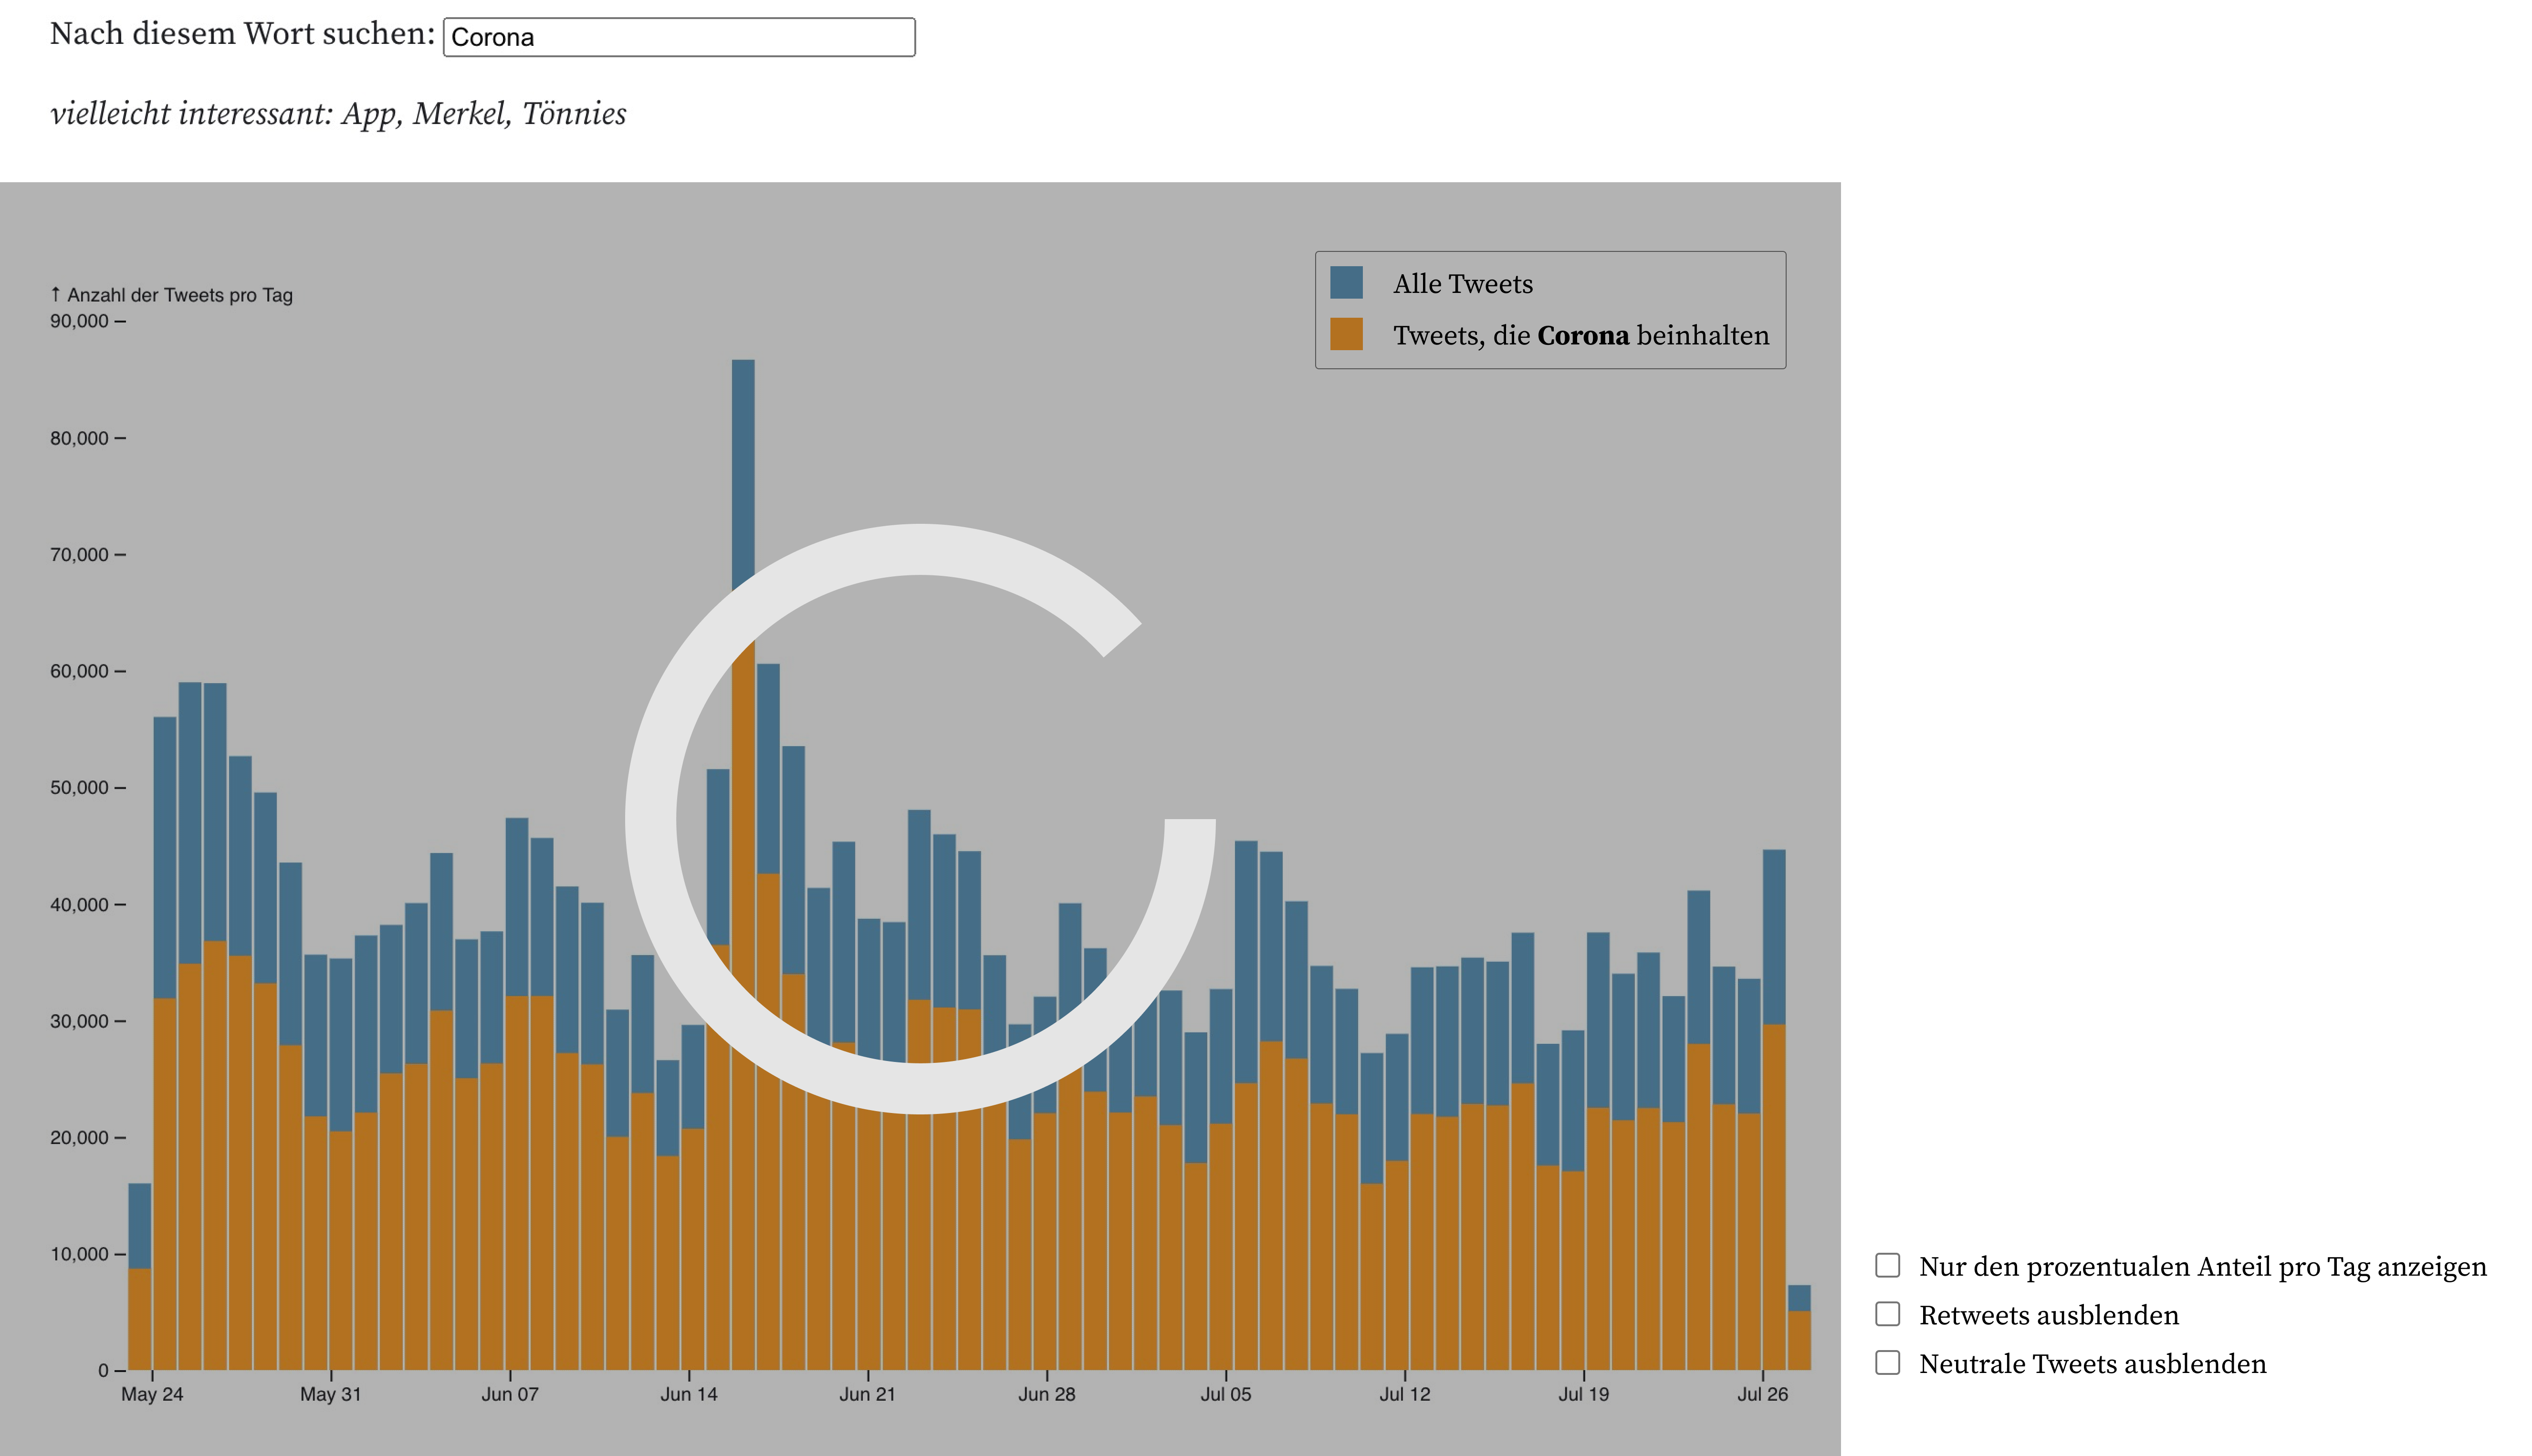
\includegraphics[width=\linewidth]{images/fetching_state.png}}
    \caption{Proposed solution to show that new data is being retrieved from the server}
    \label{fig:fetching_state}
\end{figure}

\subsection{Hindering factors: missing information}
The contents of this section are about pieces of information that participants said they would expect to interpret the data more efficiently. This information can be textual or visual: Textual information means written text, some additional explanation of how to work with the tool, or more detailed information. Visual information means, for example, more emphasis on certain aspects of the charts, or highlighted information.

\subsubsection*{Missing real-world context}
As discussed in section \ref{sec:cutForTime}, one idea that was not implemented due to time constraints was to give participants some context as to what happened on specific days based on the tweet-texts themselves. Because the calculated collocations did not yield satisfying results, this feature was not implemented for the prototype of the dashboard.

Some participants explicitly said that they would have liked to know what happened on specific days, especially when they recognized spikes in Twitter activity for a topic or spikes in the sentiment on a specific day. Further development of the tool should take this into account and, e.g., collect daily Twitter trends using the Trend API\footnote{https://developer.twitter.com/en/docs/twitter-api/v1/trends/trends-for-location/api-reference/get-trends-place, last visited on Sep. 24, 2020 \\}. This would allow participants to analyze the dataset more thoroughly. In several interviews, participants said that they would have wanted more context to understand spikes in the tweet volume or the sentiment graph. They expected this information to be present in the prototype itself, and no participant searched on the internet for further information on what happened on these days.

The Twitter trends could give at least some hints on what might have happened on these days. These trends, or trending topics, are names, phrases, or topics that are mentioned significantly more often than others. Those trending topics are fleeting, however. A study examining the trends on Twitter found that most of the trends stayed in the top 10 or even top 50 of the trending topics for less than an hour (\cite{annamoradnejadComprehensiveAnalysisTwitter2019}). This makes it necessary to aggregate the trends per day.

Showing participants the trending topics for specific days could also solve another problem that became visible during the user tests. During the free exploration in the interviews, some participants immediately had ideas that they wanted to check in the dataset (see, for example, w26b, l. 9: \say{Ich probier es mal mit Stuttgart denn da gab es ja glaub ich eine der ersten dieser Hygiene-Demos}). Others only explored the data set that was open when the notebook was first opened. This dataset showed the complete dataset, including retweets and neutral tweets, with the word filter \emph{Corona} applied. Showing daily trends could give participants ideas for how to explore the data set further.

\subsubsection*{Missing examples for the sentiment graph}\label{sec:missingExamples}
Some participants said that they found the sentiment analysis interesting. Some wished for further explanation of how the sentiment is computed and also wished to see examples of Tweets with a sentiment of +1 and a sentiment of -1 (see m23, l. 73: \say{Also klar, was das irgendwie bedeuten soll, aber... wie sieht jetzt zum Beispiel ein positiver Tweet aus oder ein negativer.}).

\begin{figure}[htb!]
    \centering
    \fbox{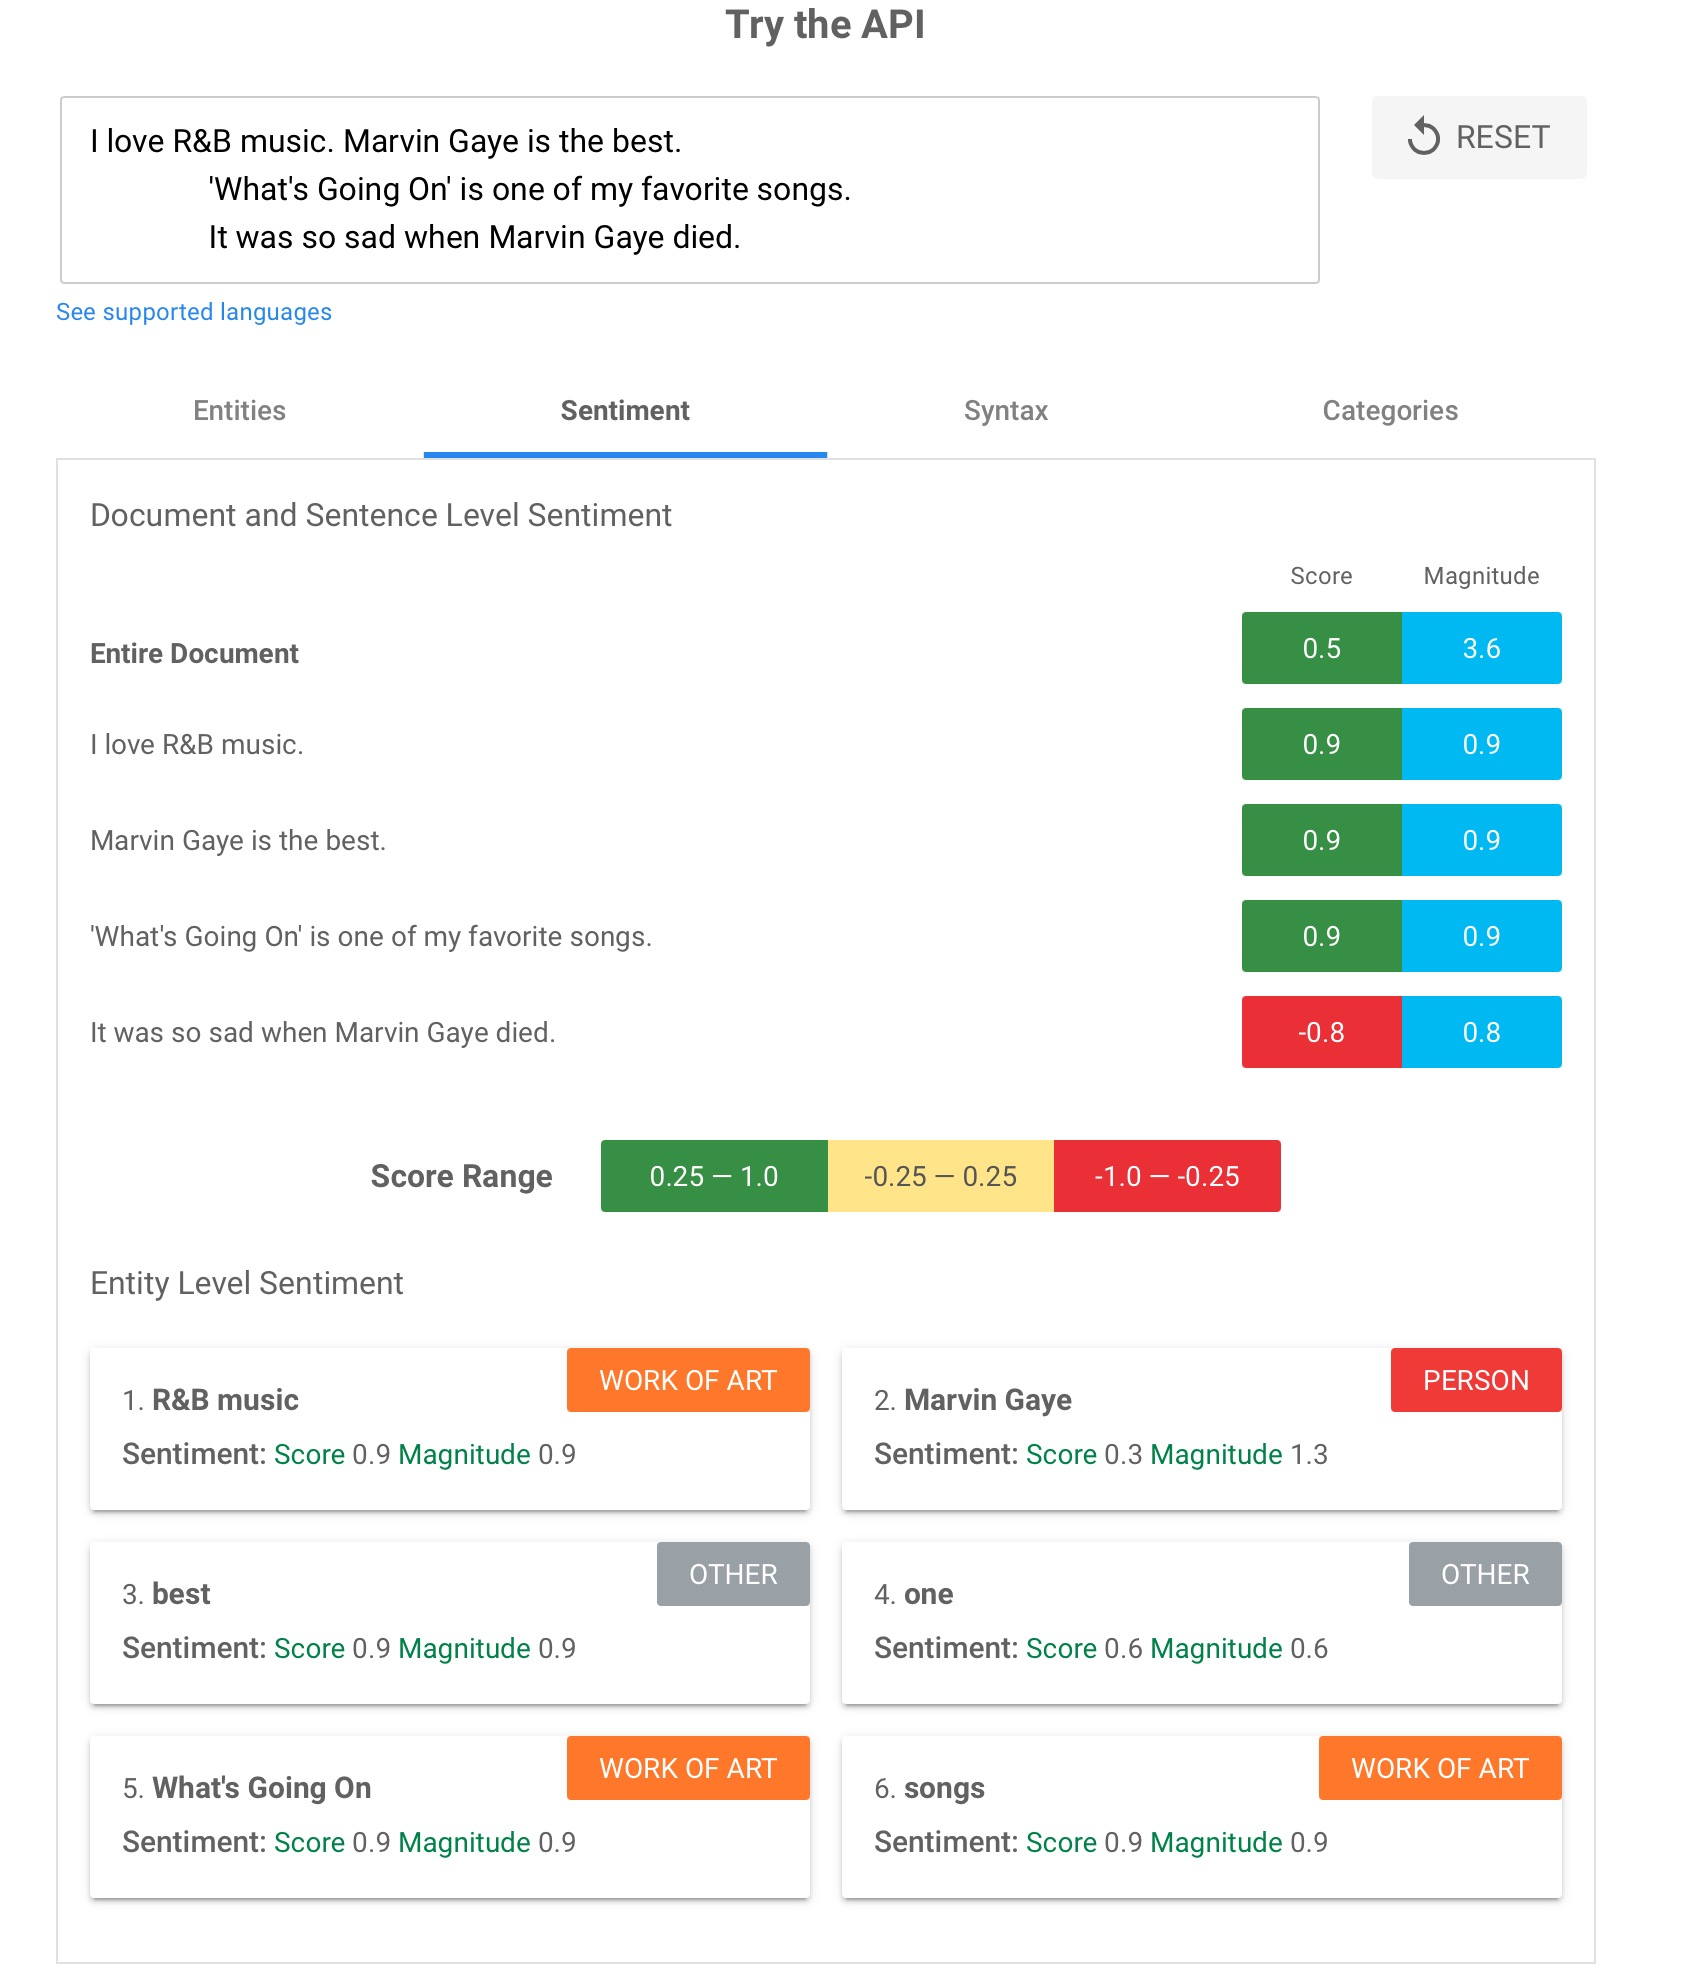
\includegraphics[width=0.8\linewidth]{images/sentiment_google.jpg}}
    \caption{The demo shows the sentiment of the full text, of the complete sentences, and for individual entities in the text.}
    \label{fig:sentiment_google}
\end{figure}

The same participant also said that he would have liked some advice on how to correctly interpret the sentiments, as well as potential pitfalls for the analysis that he should take care of. This explanation could be done in a similar form as Google explains the sentiment analysis in their Natural Language API Demo\footnote{https://cloud.google.com/natural-language/natural-language-api-demo, last visited on Sep. 24, 2020\\}, as seen in \textbf{Figure \ref{fig:sentiment_google}}. According to the participants, they would not want such an explanation for every single tweet, but rather for selected examples. This means that these examples could be hard-coded in the interface and would not have to be dynamically generated from the dataset.

At the same time, other participants said that a lengthy explanation of how the algorithm works would not have helped her and that she preferred not to have additional explanations. This means that an explanation should be an optional interface component, e.g., a tooltip near the sentiment graph. This allows interested users to access the information, while users who do not want to learn more about sentiment analysis can focus on interpreting the data at hand.

\subsubsection*{Neutral tweets-area was not marked as such}
When asked to interpret the sentiment graph, multiple participants focused on the threshold of ±0.3 for neutral tweets. This threshold was mentioned for the explanation of the \emph{neutral Tweets}-toggle and is, as discussed in chapter 2, a common threshold to differentiate between neutral Tweets and Tweets that carry an opinion. The participants looked for peaks above or below ±0.3 to find days where the discourse on twitter was especially emotional. This could be facilitated by marking this area in the chart itself, similar to how the 0-baseline was marked. An example for this can be seen in \textbf{Figure \ref{fig:sentiment_neutral_area}}.

\begin{figure}[h!tb]
    \centering
    \fbox{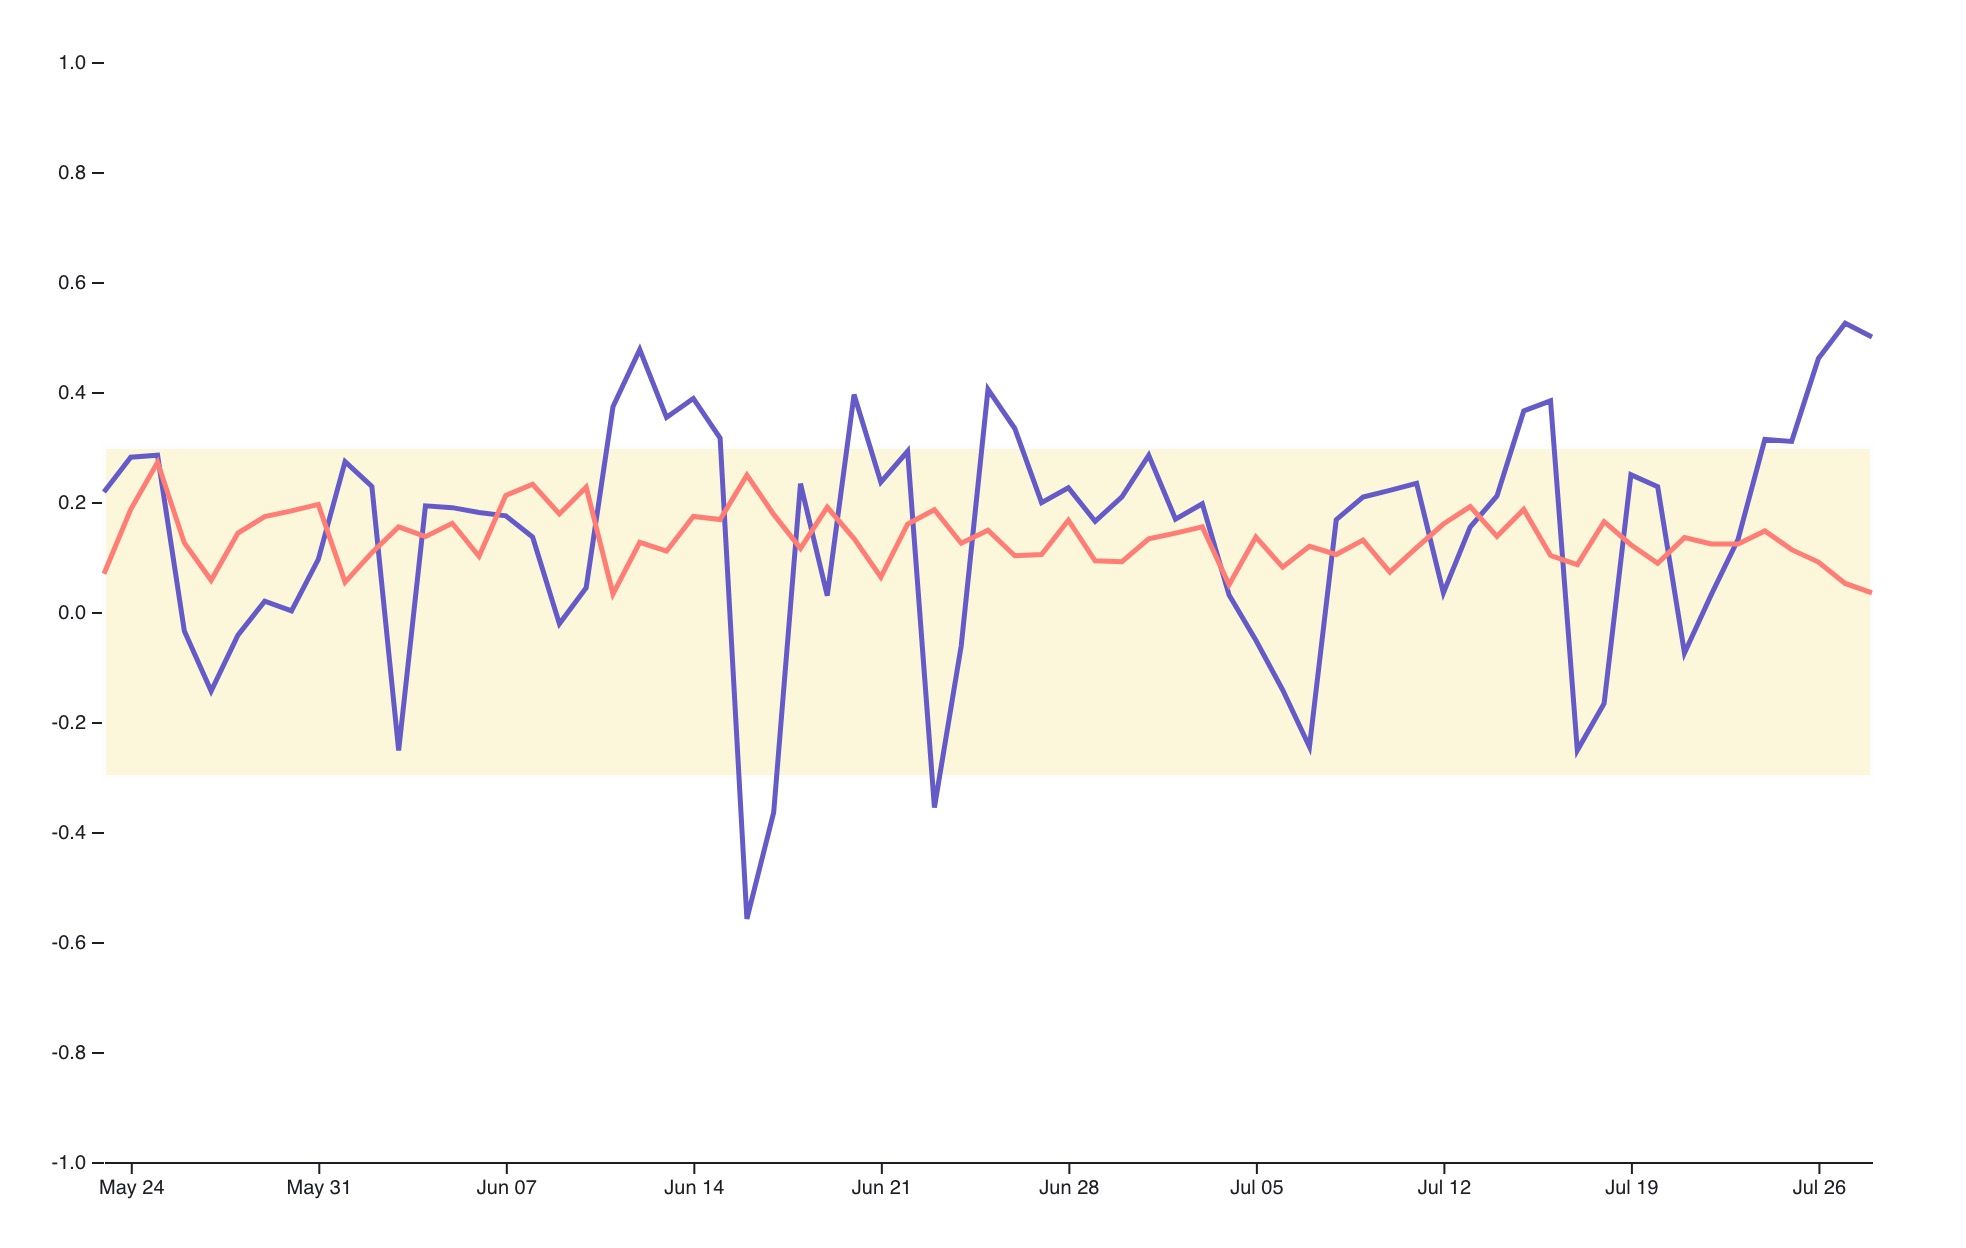
\includegraphics[width=0.98\linewidth]{images/sentiment_neutral_area.jpg}}
    \caption{The area containing the neutral tweets is marked, making it easier to identify spikes above or below the threshold. The screenshot shows the data when filtered for \emph{Drosten}.}
    \label{fig:sentiment_neutral_area}
\end{figure}

\subsection{Hindering factors: Technical limitations}
This section discusses findings from the interview where technical limitations hindered participants from solving tasks. Some of these limitations were conscious trade-offs for this prototype version. Nonetheless, these issues should be addressed if a tool based on this prototype should be further developed.

\subsubsection*{Fixed data set} \label{sec:fixedDataSet}
The fixed data set came up in one interview where the participant tried to scroll the data set to reveal even more days. This revealed one of the biggest disadvantages of using Twitter's streaming API to collect tweets in real-time (see section \ref{sec:fetchedData}). Using this method guarantees the most complete data set on the free tier of Twitter's API, at least from the time the data collection is started. The downside is that using this API makes it impossible to access past tweets. Users of the tool have to recognize a potentially interesting topic very early, start the data collection, and then wait some time until enough data has been gathered.

Using the paid API to access Twitter's archives could solve this problem, at least in parts. The paid access to Twitter's archives gives access to the past 30 days of activity on Twitter, which could give a 'headstart' to the data collection. For a final version of this tool, a combined approach could be possible: using the real-time data collection of a specific topic with the streaming API, and simultaneously fetching the last 30 days of Twitter activity to this topic. This would mean that users would be able to analyze the past month of tweets directly from the beginning of the data collection, eliminating the need to wait some days before they can gather meaningful results from Twitter.

If this approach would be used, the data collection pipeline would have to be modified further. In the current implementation, the sentiment of a tweet is computed synchronously when the tweet is sent to the collecting app by the streaming API. The data sent by the Twitter archive may be too big to compute the sentiment synchronously. In this case, users should get a message that the sentiment is being computed, but that they can already start analyzing the volume graph.

Allowing users to explore a bigger data set could mean that the way the data set is presented has to be changed. One example of showing a data set that spans multiple months can be seen on Spiegel Online (\cite{merlotCoronavirusBrasilienManaus2020}).

\begin{figure}[htb!]
    \fbox{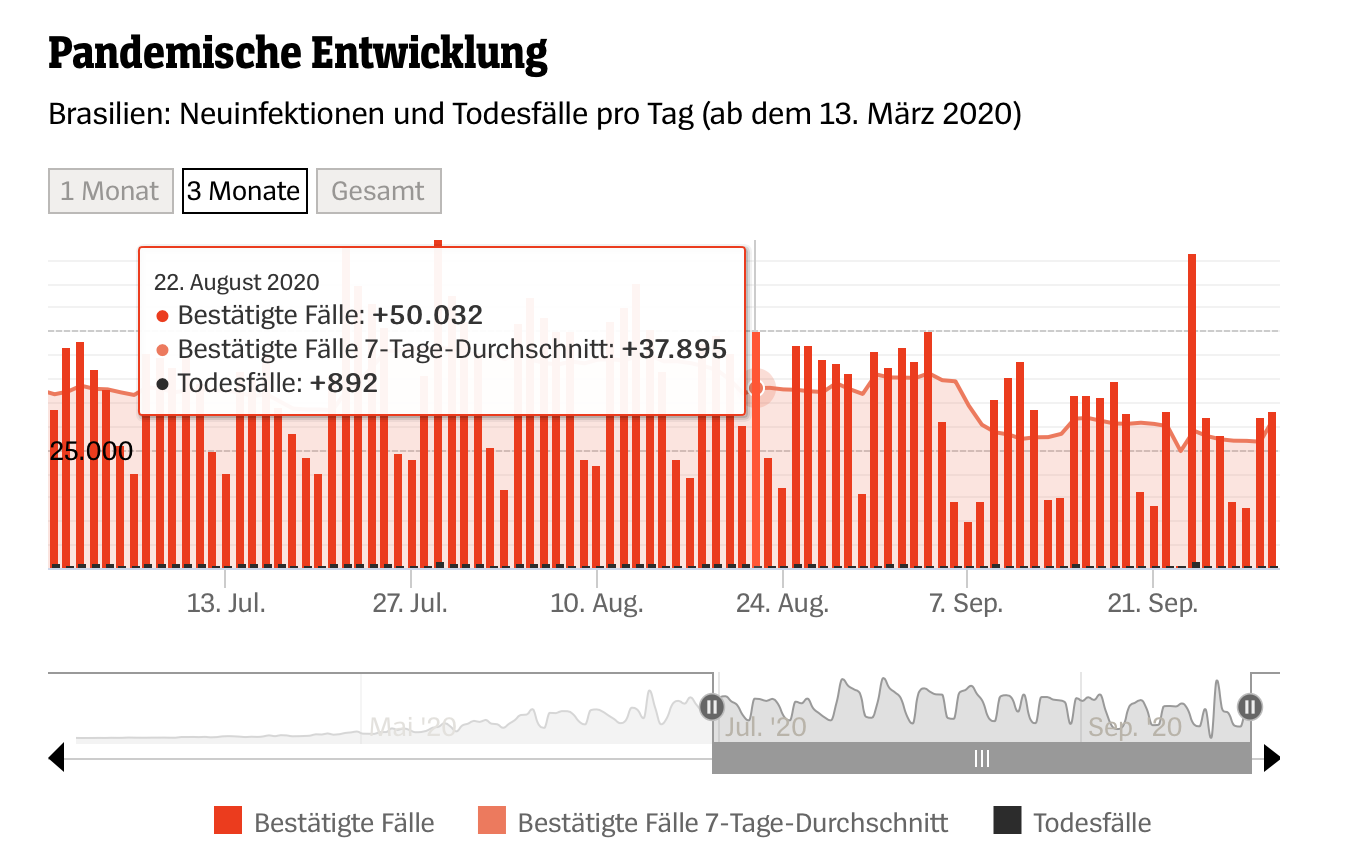
\includegraphics[width=\linewidth]{images/spiegel_visualization.png}}
    \caption{A coronavirus visualization from Spiegel Online. The buttons on top select the time frame that should be displayed. The scroll bar below the chart allows users to move the viewport to explore other parts of the dataset. Users can also drag the size of the scroll bar to change the time frame that is displayed. Taken from \cite{merlotCoronavirusBrasilienManaus2020}.}
    \label{fig:spiegel_visualization}
\end{figure}

The chart showing the new infections and corona-related casualties in Brasil can be manipulated by users in different ways:
\begin{itemize}
    \item Buttons on top of the chart let users switch the scope of the data set between 1 month, 3 months, and the whole data set.
    \item The scroll bar allows users to move the selected time frame. This means they can see data from the last three months starting today, from the last three months starting next week, or wherever users move the scroll bar.
    \item The scroll bar can also be resized. By doing this, users can choose a time frame other than the default three options.
\end{itemize}

Similar to what was already mentioned in this discussion, the visualization from Spiegel Online also has a tooltip which shows more detailed information and a visual legend that explains the colors in the graph. 

\subsubsection*{Basic word filter}
Another problem that needs further technical work is how the word filter works. The current implementation acts as a case-insensitive filter that looks for parts of words. This means that, if a user enters \emph{App}, tweets containing these sorts of texts will be found:

\begin{itemize}
    \item I like this \textbf{App} a lot
    \item Whats\textbf{App} collects your data
    \item What kind of video \textbf{app} would you recommend?
    \item I'm not angry, just dis\textbf{app}ointed
\end{itemize}

This is different from how search engines, like DuckDuckGo, Google, or Bing, work. These engines use a so-called \emph{fuzzy search} which not only looks for the word itself, but also catches typographic mistakes, looks for synonyms, and so on.

Using a fuzzy search would allow users to explore the database more efficiently. During testing, for example, it was shown that typographic mistakes in the filter field would mean that little to no results were found, assuming that most of the Twitter users wrote the word correctly. The participant in question thought that there was not a lot of Twitter activity about the specific topic she was interested in. After one participant was told to correct the typo, she noticed an interesting pattern in the tweet activity and was able to interpret the data further. This means that it could be helpful to implement a fuzzy search to further develop the prototype.

\subsubsection*{Tooltips for the sentiment graph}
During the user tests, the participants expected to find tooltips for both graphs once they found the tooltip in the volume graph. This means that tooltips should either be used globally for all visualizations, at least where the additional information provided by the tooltip adds to the value. Alternatively, no tooltips at all could be used. As the tooltip in the volume graph helped participants to further explore the dataset, it should be kept for all the visualizations. Those tooltips would also satisfy \citeauthor{shneidermanEyesHaveIt1996}'s \emph{details-on-demand} by showing additional information when the user wants to see them, instead of cluttering the interface. Because of the way the tooltips were implemented in this prototype, they could not be added to the sentiment graph. More on this limitation can be found in Section \ref{fw_tooltips}.


\clearpage
\section{Method reflection}
This section will discuss the methods used for this master thesis. While the results are generally convincing, there is still room for improvement in further studies.

\subsection*{Using qualitative content analysis could only answer parts of the research question}
One of the biggest issues for the author of this study is that the focus of the study and the focus of this written-out thesis do not fully overlap. The study began as a feasibility analysis that aimed to find out if it is possible to collect large amounts of tweets and show them in such a way that laymen can interpret the data. In this initial state, the study consisted of two parts:

\begin{enumerate}
    \item The automated collection and storage of every German tweet to a specific topic---in this case, tweets related to the Coronavirus,
    \item and an easily accessible visualization of these tweets which can give insight to people who are laymen when it comes to analyzing big data
\end{enumerate}

One of the study's goals was to test several approaches on how to implement these two parts. To evaluate the outcome of this study from a communications science-perspective, an additional interview study based on Mayring's approach to qualitative content analysis was conducted. The results reported in this thesis are mostly based on the findings of this interview study.

However, this study did not further examine the quality and feasability of the code that was written. While the study showed that there \emph{is} a possibility to automatically collect and store tweets with certain filter criteria, it did not give additional insight in \emph{how} to do it. 

Focusing on the qualitative content analysis gave insights on what laymen expect from a data visualization and what helps them to analyze data. It did not answer the questions if the method to collect and store the tweets and to visualize the data set were appropriate.

\subsection*{Streaming API made it impossible to take Likes into account}
One of the possible problems of collecting the data the way they were collected is that Likes could not be taken into account for the analysis of the tweets. Studies have shown that Likes are strongly linked to actual engagement and support, e.g., during congressional elections (\cite{macwilliamsForecastingCongressionalElections2015}). This hints at the importance of Likes to measure the general public's approval of specific tweets. In the current implementation, the volume of the tweets strongly affects the sentiment analysis: if many negative tweets are sent on a specific day, the overall sentiment on that day will go down. This holds true the other way around as well. Many positive tweets affect the curve so that the daily average goes up.

This means that, in theory, a bot army could flood specific topics with very negative tweets. Even if not a single person saw these tweets, or interacted with them, these tweets would affect the reported overall sentiment. If the Likes of a tweet could be collected as well, users could, e.g., filter for tweets with at least 5 likes. This would filter out the tweets which did not drive engagement on Twitter.

On the other hand, this approach would bring additional problems:
\begin{itemize}
    \item Tweets from smaller accounts would be filtered out, even though these accounts are not necessarily part of a bot network.
    \item Filtering out tweets that have less than an arbitrary number of Likes distorts the data set in some way. While they might paint a more accurate picture of what society thinks by filtering out automated, nearly invisible tweets, this could also silence the influence of people without celebrity or influencer status. Seeing that Twitter is a grassroots medium that allows people to make their voices heard regardless of their social status (\cite{passmann2019alte}), a carelessly implemented filter option could silence those voices.
    \item Collecting a tweet's Likes requires either the usage of the archive API or a script that fetches the Likes of a tweet a specific time after it was collected, e.g., three days after initial collection. This is necessary because the streaming API sends a tweet to the collecting script almost immediately after it was sent. This means that every time the streaming API sends a tweet, its number of Likes should be 0.
\end{itemize}

Future studies could focus on addressing these issues and finding a way to make the dataset, on the one hand, more reliable---e.g., by filtering out bots---while on the other hand keeping the open culture of Twitter in mind and not silencing the voices of everyday people.

\begin{itemize}
    %\item Streaming API was the better option on the free tier. But this solution is not flexible enough to see how different topics get discussed on Twitter: the data collection ran over 2 months, and this might not be feasible. (braucht eigentlich nicht mehr gemacht werden)
    \item Accessibility issues: too much reliance on colors alone. It would have been better to also include texture patterns. Both color and patterns are qualitative nominal variables, so they can encode the same information (\cite[1860]{bornerDataVisualizationLiteracy2019}).
    \item Using \emph{Shape Up} to plan the development of the tool worked well. It is possible, however, that the clear distinction pipeline---d3-visualizations---writing the thesis meant that some parts of the study, like the pipeline, took more time than necessary.
    \item The participants in the interview study were mostly students. This was partly because of the ongoing Covid-19 pandemic, which made it necessary to use online conferencing software to recruit the participants and conduct the interviews with them. Face-to-face interviews with a more diverse group of participants can yield further results. This should be considered for future studies.
    \item Using Observable sped up the development process and was the right choice for the prototype. For a final product, however, the limitations of Observable are too severe, especially when using databases. Notebooks with databases require permissions to be set up, and for this users need to create an Observable account and join the team workspace where the notebook is located. Instead of using Observable, users should be able to use a web tool without logging in. One example of a data analysis tool on the web is \emph{Blacklight}\footnote{https://themarkup.org/blacklight/}, where users can scan other web pages for trackers.
\end{itemize}


\clearpage
\section{Conclusion}
The impact of social media on society, politics, and personal well-being is not likely to decrease in the future. This relationship between social media and its users is an asymmetrical one, however: Users cannot gain insight into how social media works, how the algorithms select contents, and most importantly  how social media might skew one's perception of reality. Already today, this poses a real threat to society as the engagement-driven recommender algorithms support a rise of populism (\cite{groshekHelpingPopulismWin2017}).

This study examined ways to automatically collect, process, and store large amounts of Twitter data. Then, using visualizations, this data set was made accessible to laymen. Using such a tool to examine how specific topics are discussed on Twitter makes it easier for users to understand what is going on in the world. Tools like the one presented in this study can even be seen as the future of journalism: not a one-way street of pre-analyzed data, but rather giving readers \say{the tools to hold institutions in your life accountable for their choices.} (\cite{angwinMakingPrivacyPersonal2020}).

The visualizations were tested in user studies to see if laymen can indeed gain meaningful insights from the visualizations. While some potential for improvement was found, the results generally hint at laymen indeed being capable of reading visualizations, as long as some rules and guidelines are followed.


%- the impact of social media on society, politics, and well-being is not likely to decrease in future years. Meanwhile, users of social media cannot get an objective view of the network, as they mostly see contents that are chosen by an engagement-driving algorithm. This could pose a real threat to society and a rise of populism (Groshek2017).

%- this study examined ways to automatically collect, process, and store large amounts of Twitter data and make such a dataset accessible to laymen. This could give them the tools to examine how specific topics are discussed on social media, making this less opaque.

%- The visualizations were tested in user studies to see if laymen can gain meaningful insights from the visualizations.

%- the user study showed that laymen could gain insight from these visualizations while analyzing further improvements that future studies could focus on.

\newpage
\printbibliography

\end{document}
